\begin{figure}[H]
    \centering
    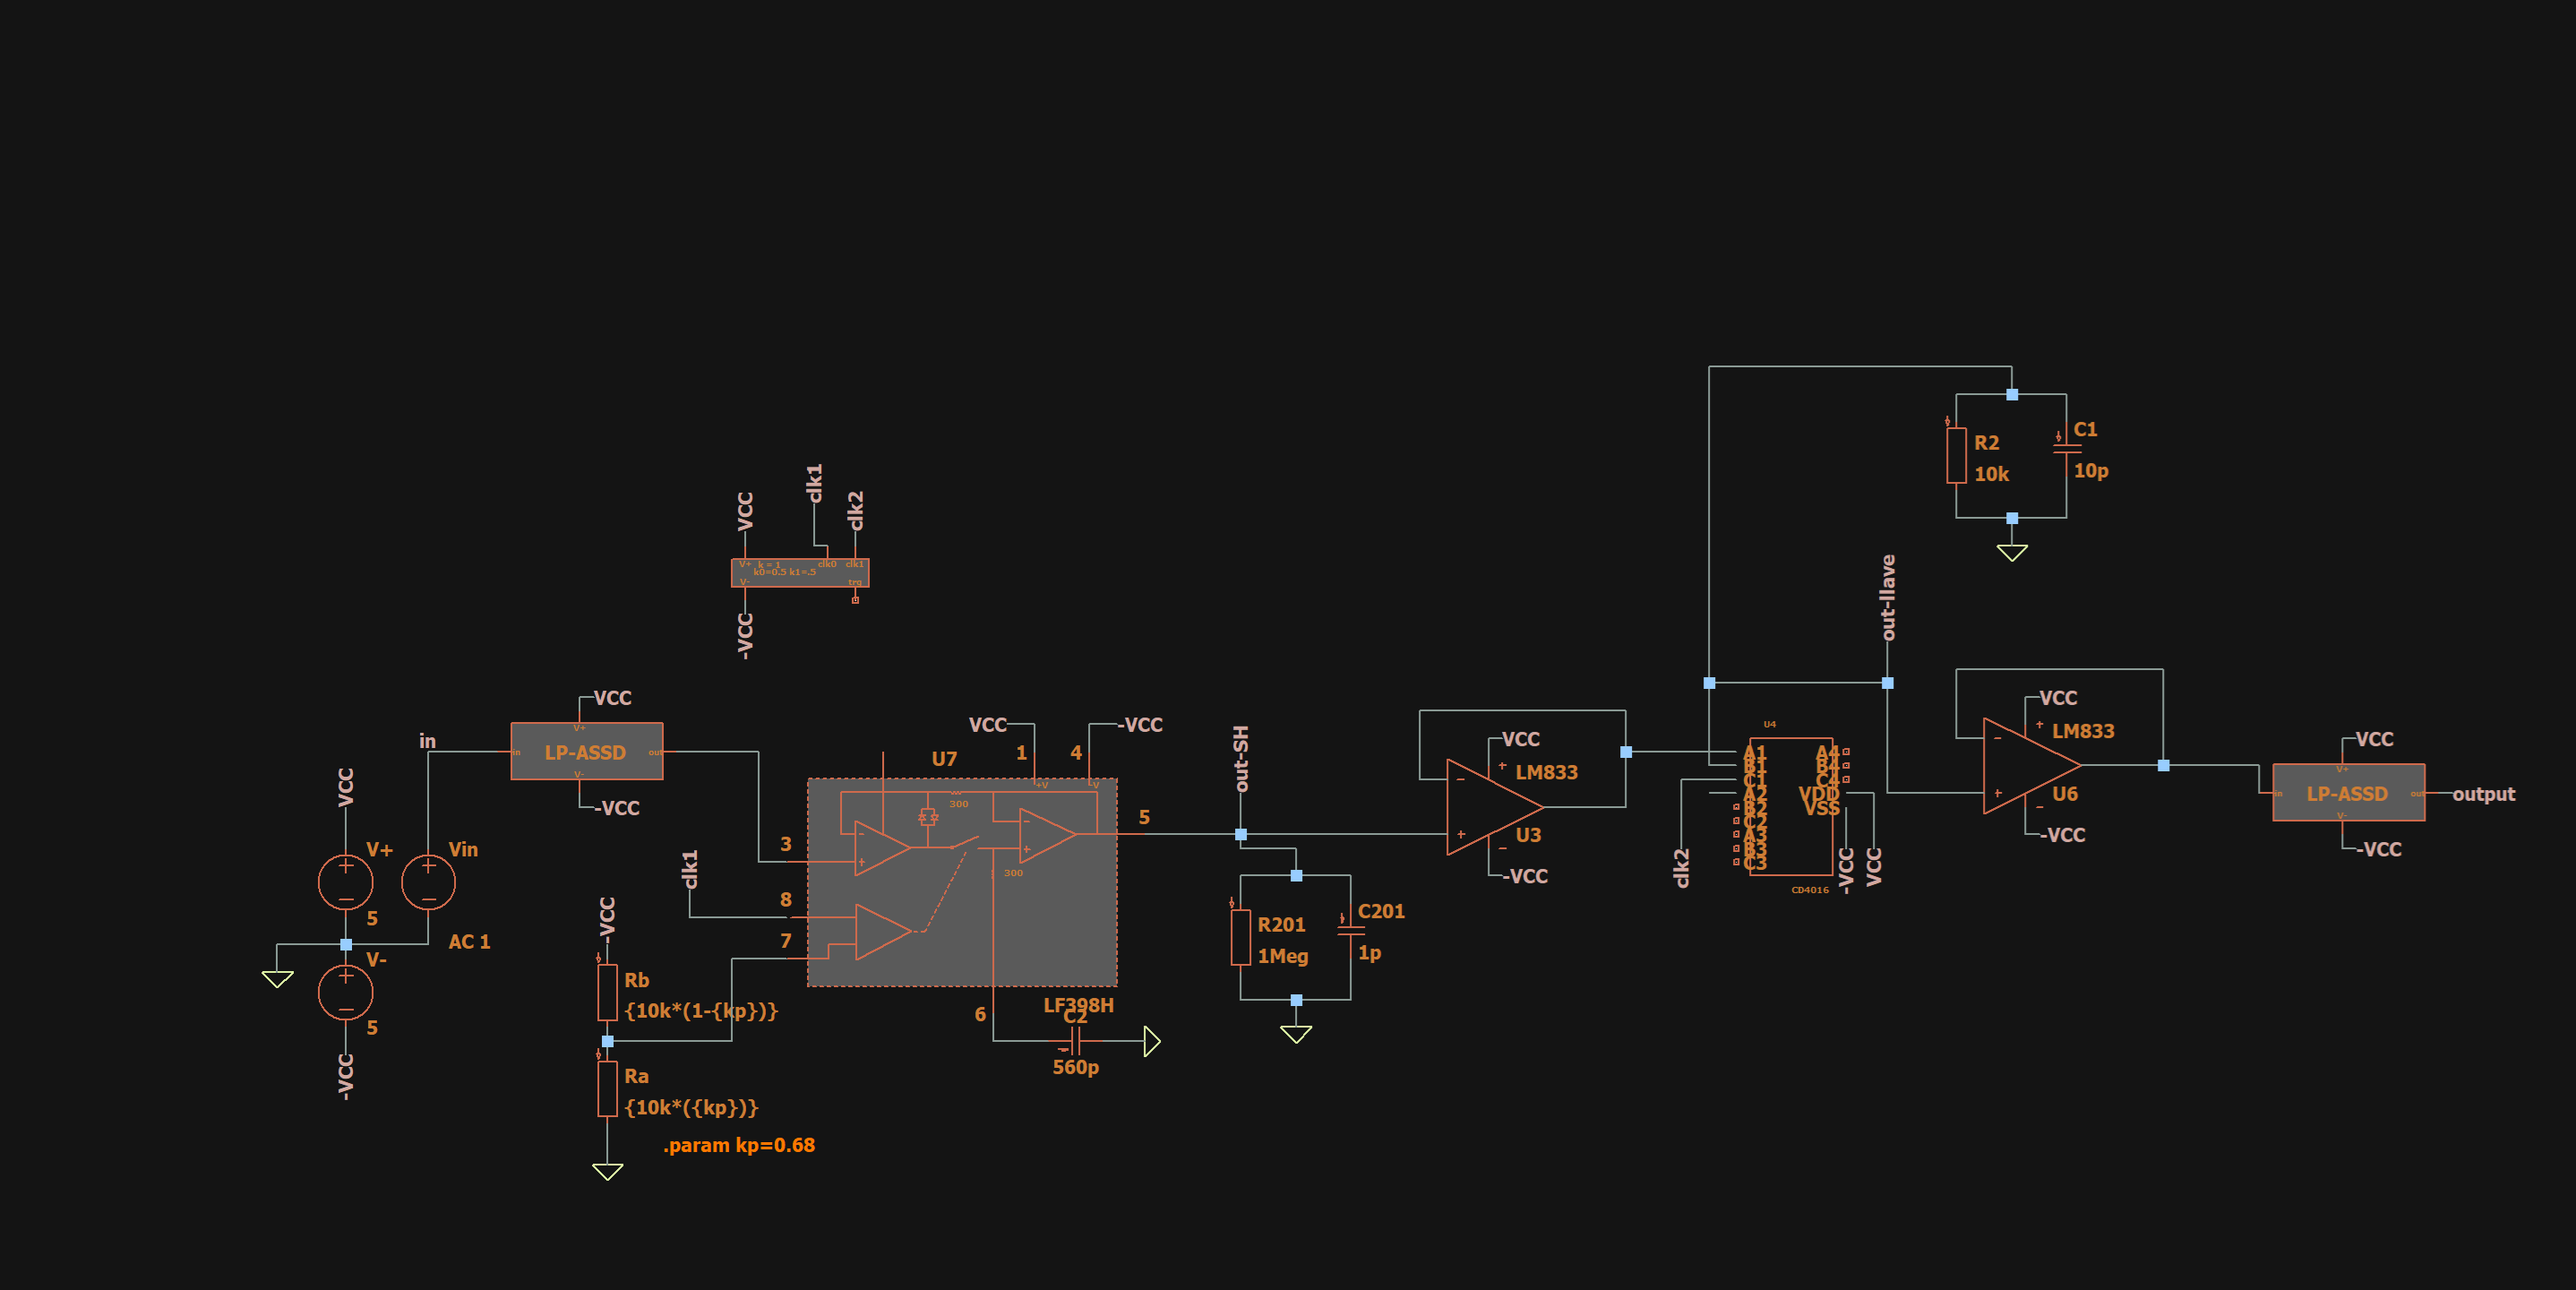
\includegraphics[width=0.9\linewidth]{Imagenes Nacho/EsquemaLatex.png}
    \caption{Circuito completo de simulaci\'on en LTSpice}
    \label{fig:EsquemaLatex}
\end{figure}


Para garantizar el correcto funcionamiento del circuito, se opt\'o por simular por m\'odulos el circuito, creando componentes de los mismos una vez que su funcionamiento era reconocido para un esquema final como se observa en la figura \ref{fig:EsquemaLatex} . 

\subsection{Filtro Low-Pass}
El componente "LP-ASSD", encapsula un filtro pasabajos de 6to orden Cauer con frecuencia de corte en $80kHz$. Se decidi\'o por 3 celdas SEDRA en cascada, debido a su facilidad de implementaci\'on y experiencia previa con los mismos. Luego de encontrar los polos y zeros de cada celda y evaluar las etapas de ganancia para evitar saturaci\'on entre etapas, se simul\'o el orden y condiciones de las mismas para garantizar su funcionamiento optimo. A continuaci\'on los resultados:

\begin{figure}[H]
    \centering
    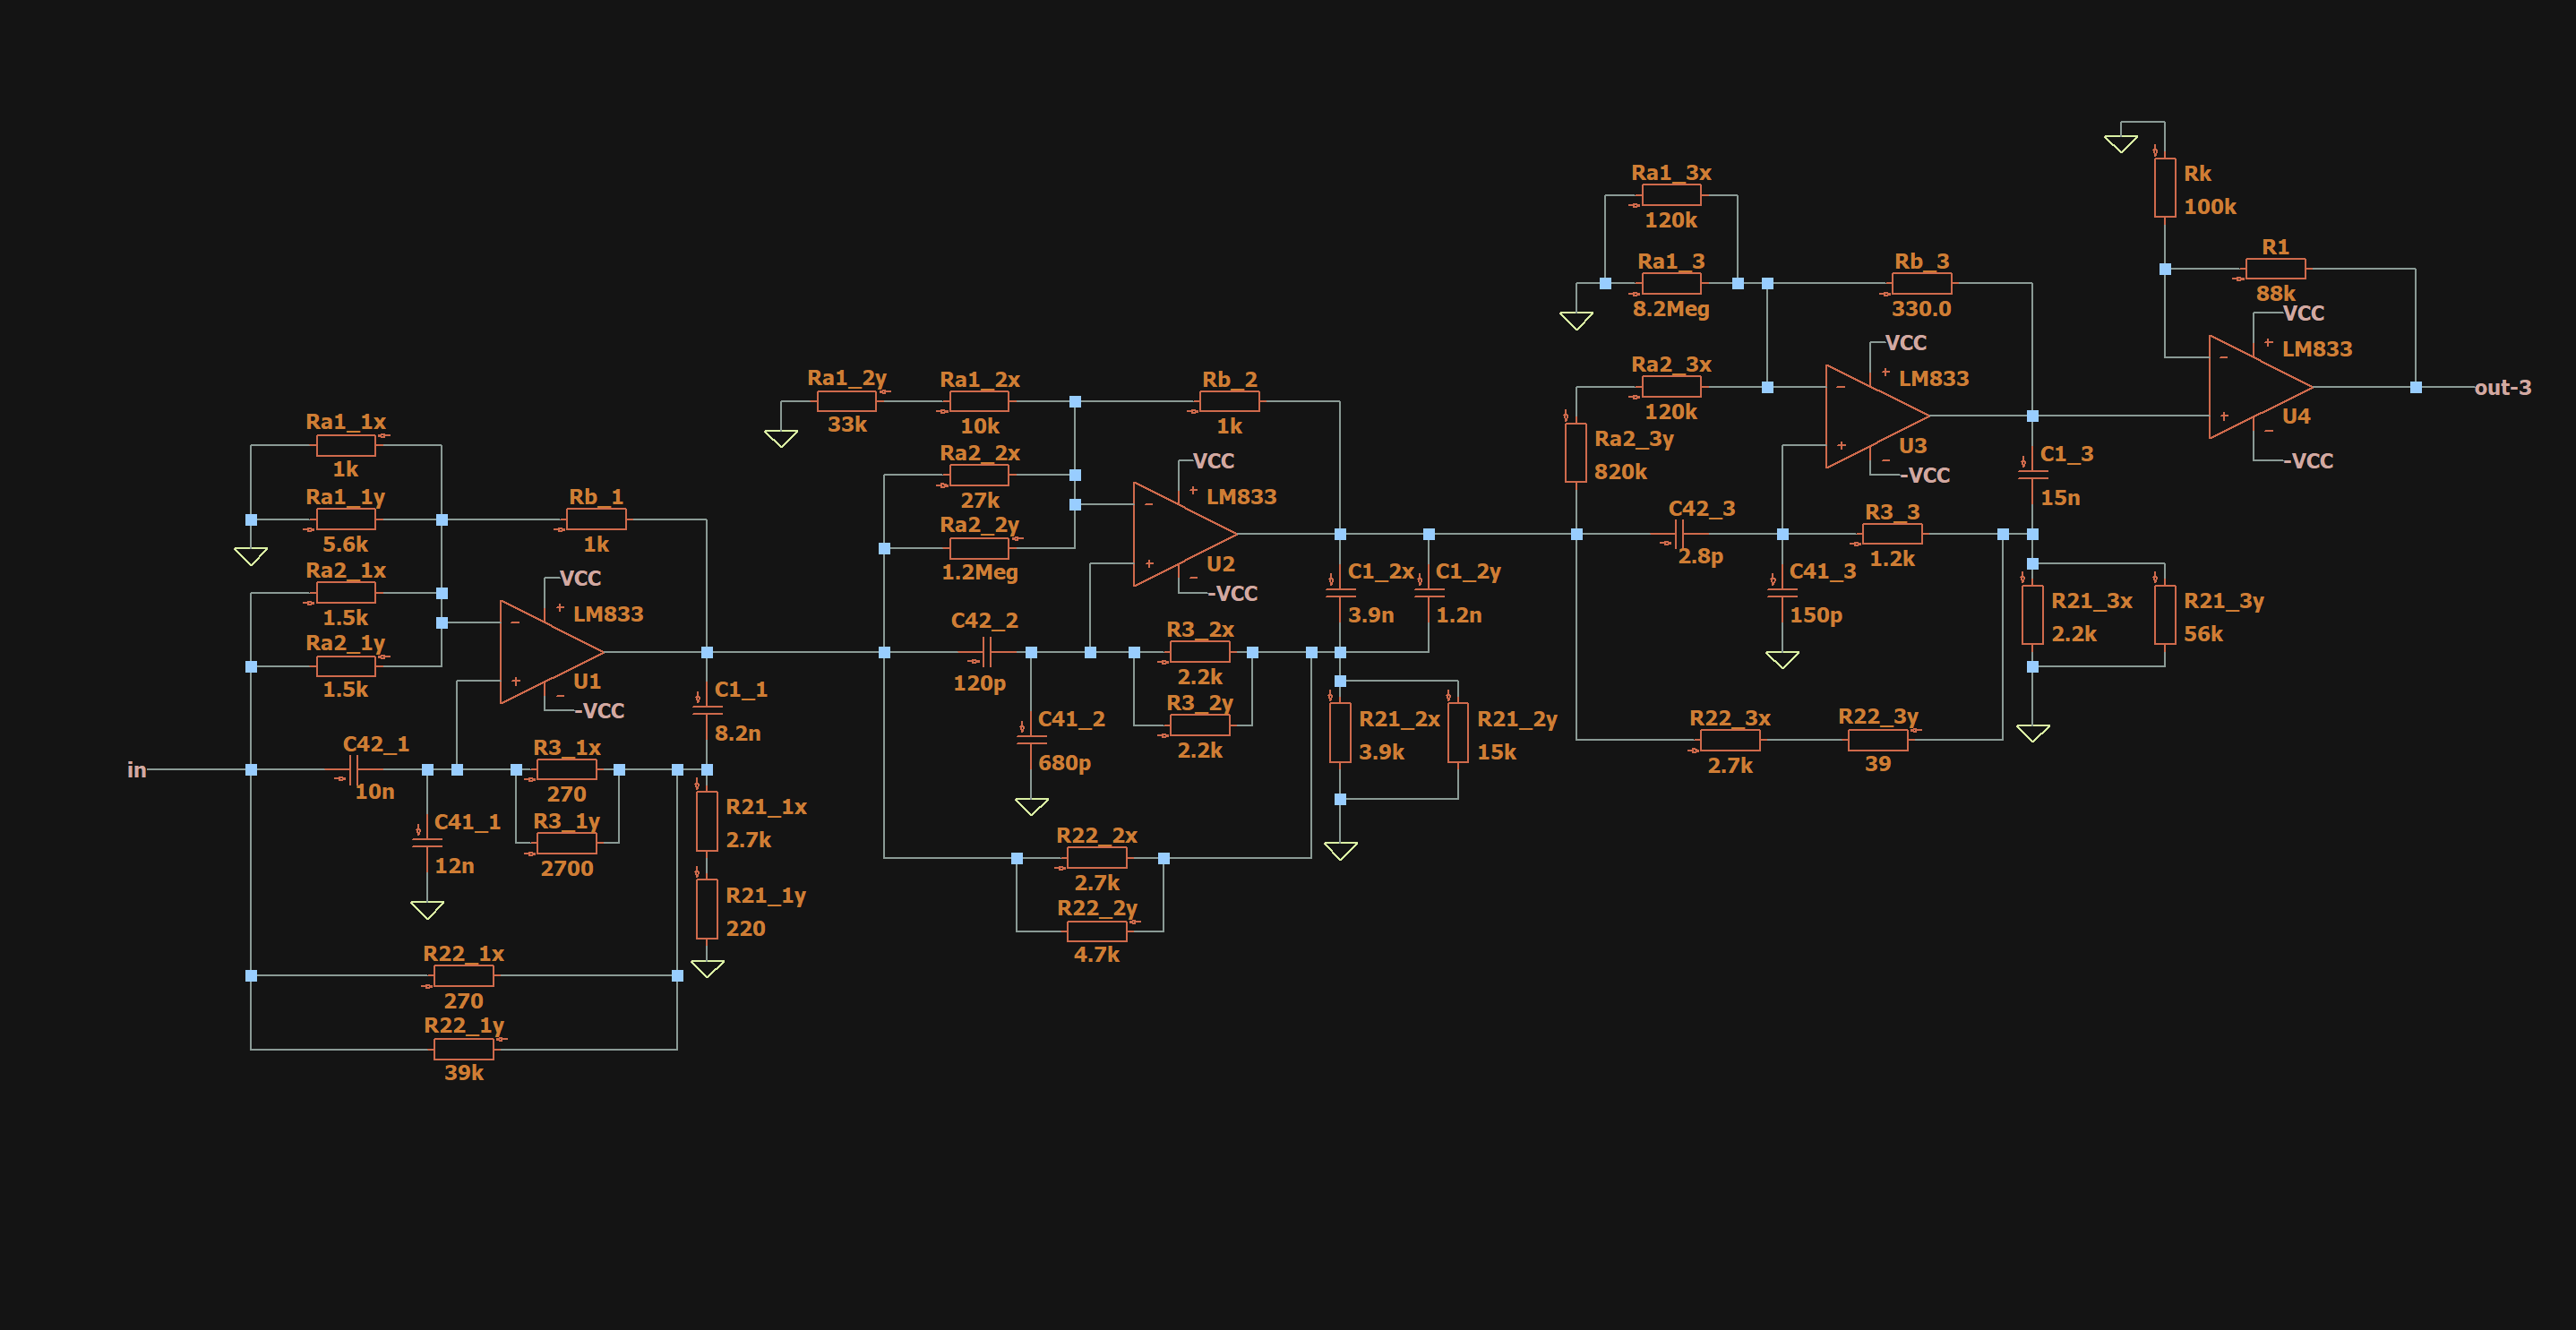
\includegraphics[width=0.8\linewidth]{Imagenes Nacho/EsquemaLatexLowPass.png}
    \caption{Celdas SEDRA en cascada como filtros Low-Pass}
    \label{fig:EsquemaLatexLowPass}
\end{figure}

\begin{figure}[H]
    \centering
    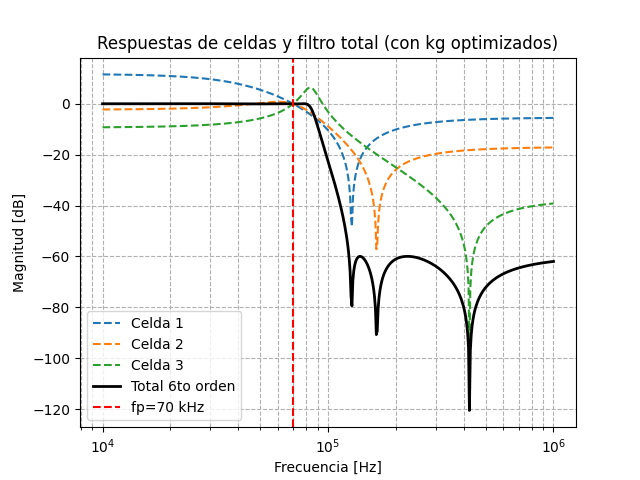
\includegraphics[width=0.8\linewidth]{Imagenes Nacho/Python.png}
    \caption{Evaluaci\'on de Etapas de Celdas Individuales}
    \label{fig:Python}
\end{figure}

\begin{figure}[H]
    \centering
    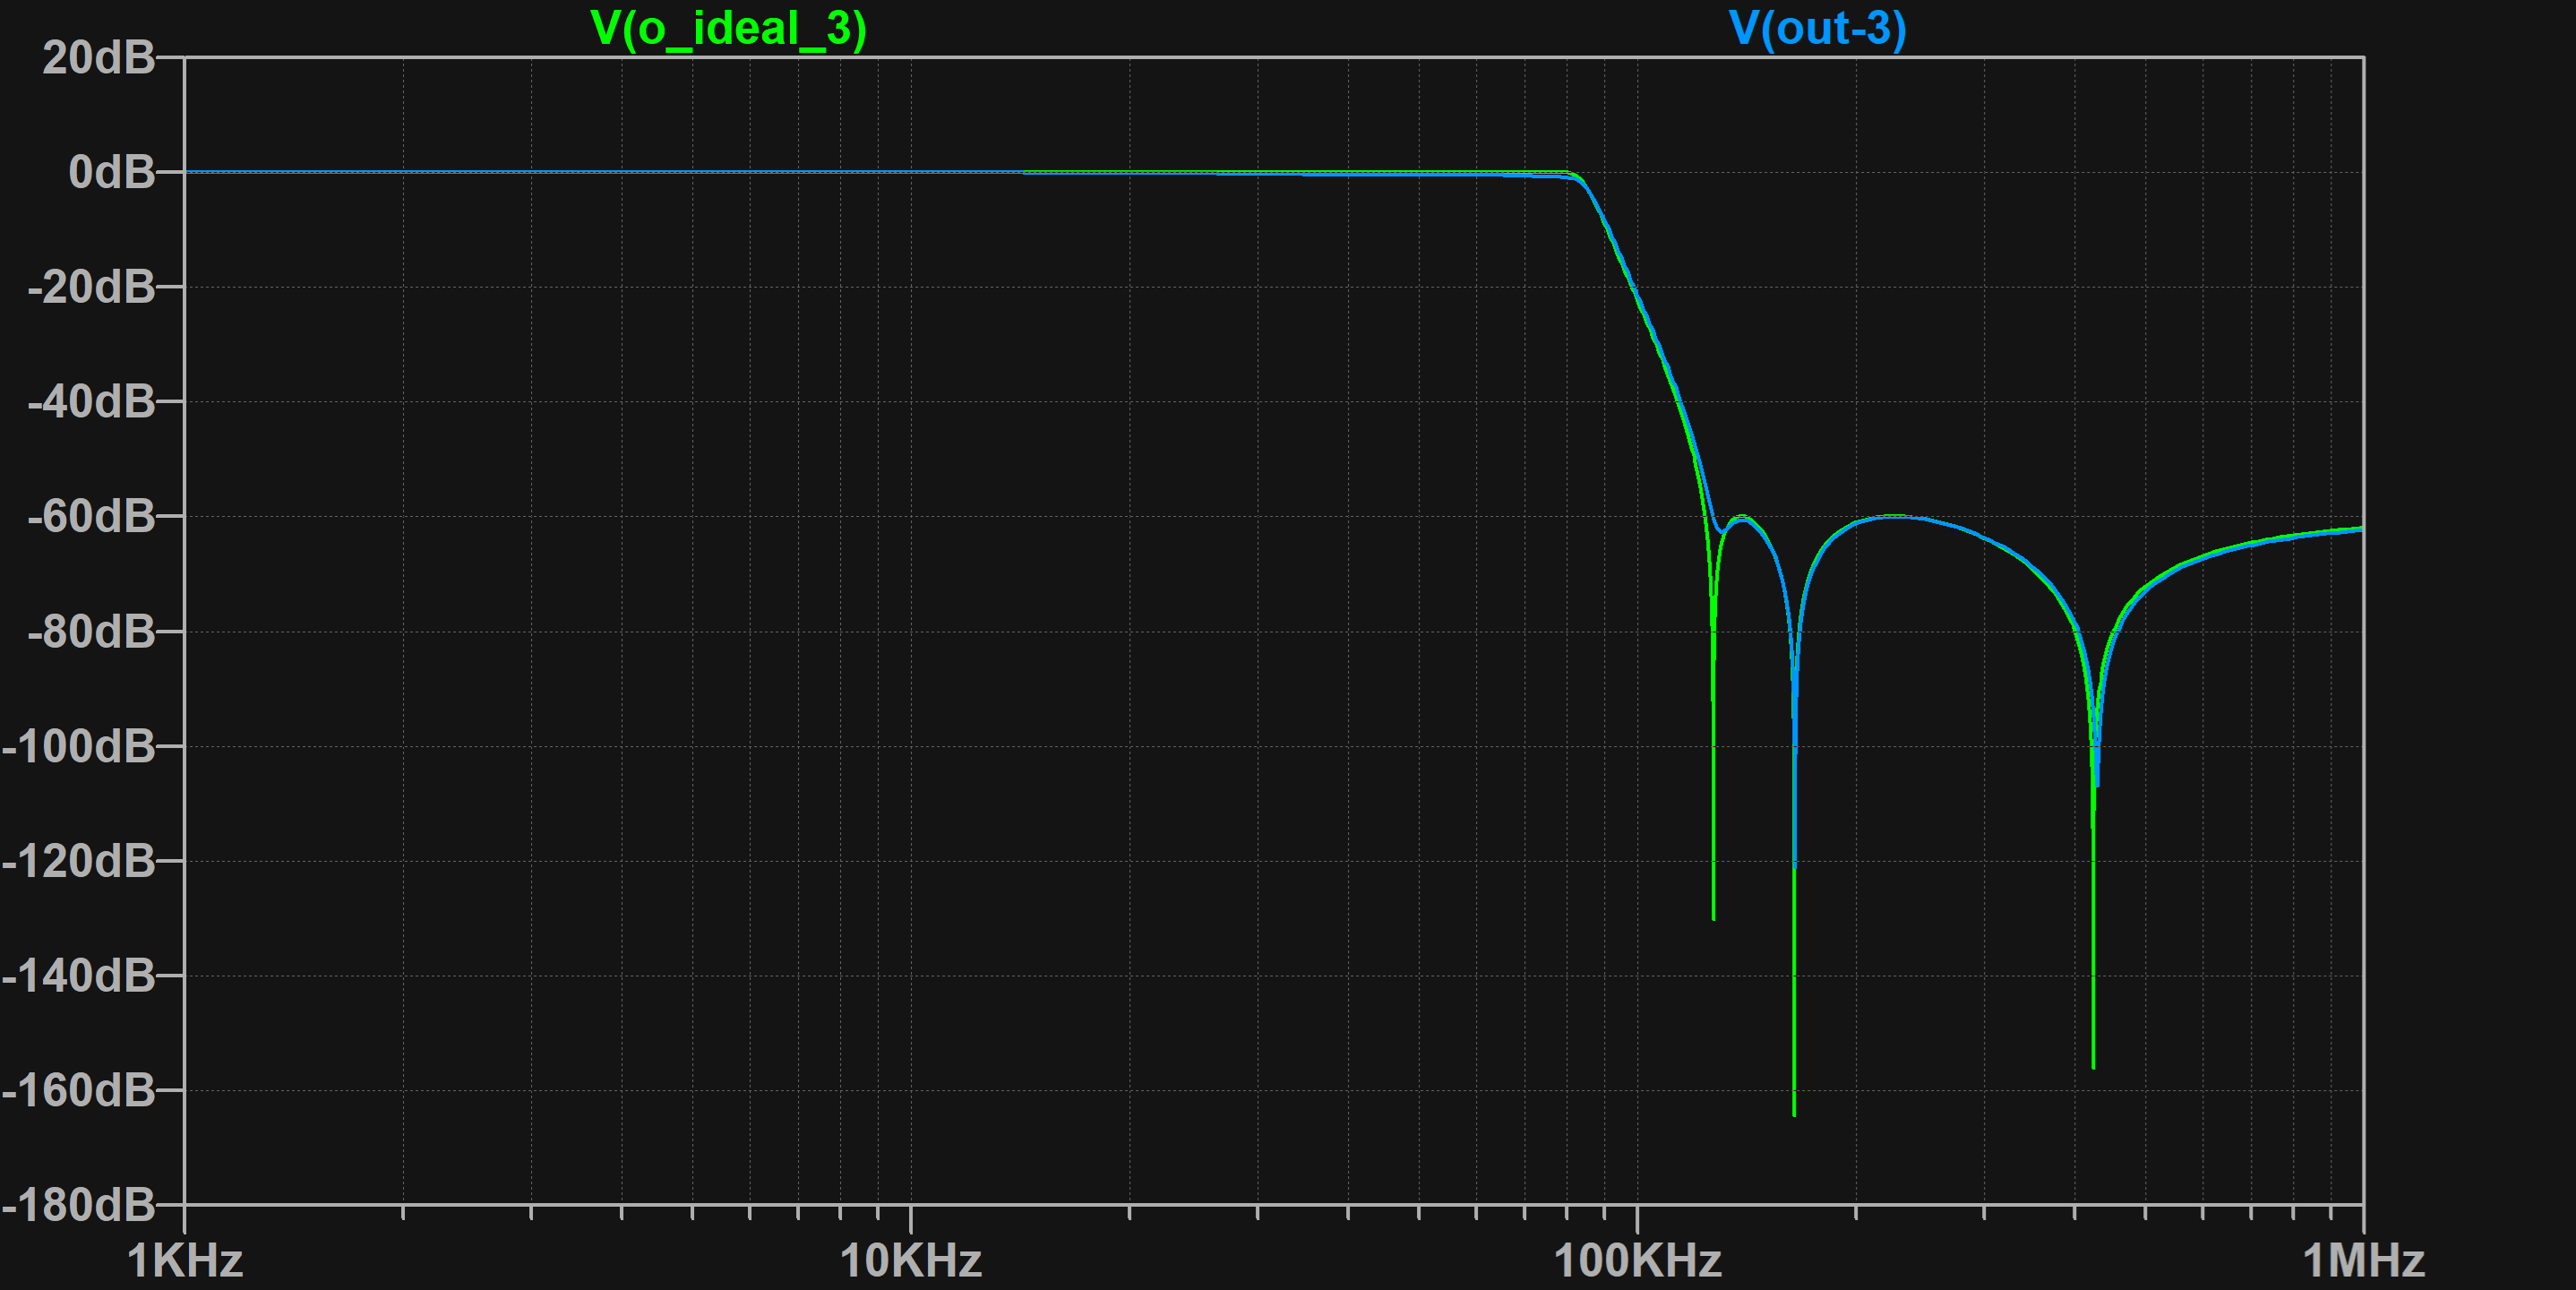
\includegraphics[width=0.8\linewidth]{Imagenes Nacho/LowPassFitler.png}
    \caption{Filtro Low Pass: Funci\'on ideal vs Implentacion}
    \label{fig:LowPassFitler}
\end{figure}

un problema que tuvo este filtro en su implementaci\'on, es que la primera etapa posee una impedancia de entrada muy, por lo que se debi\'o colocar un buffer. Adem\'as, La ganacia en la vida real se desvia de la expectativa por las tolerancias de los componentes, por lo que se debe colocar una etapa de ganancia variable para garantizar que no se atenuen las frecuencias deseadas.

\subsection{Oscilador}

El pequeño componente que se puede apreciar en la figura \ref{fig:EsquemaLatex}, encapsula el circuito generador de clock. El mismo requiere unicamente como entrada las fuentes de alimentaci\'on, con las salidas siendo la carga y descarga de un capacitor ($trg$), clock 1($clk1$) y clock 1($clk2$). Variando $k$ se ajusta la frecuencia de los clocks podiendo llegar hasta los $250kHz$ y ajustando $k1$ y $k2$ el duty de los respectivos clocks. 

\begin{figure}[H]
    \centering
    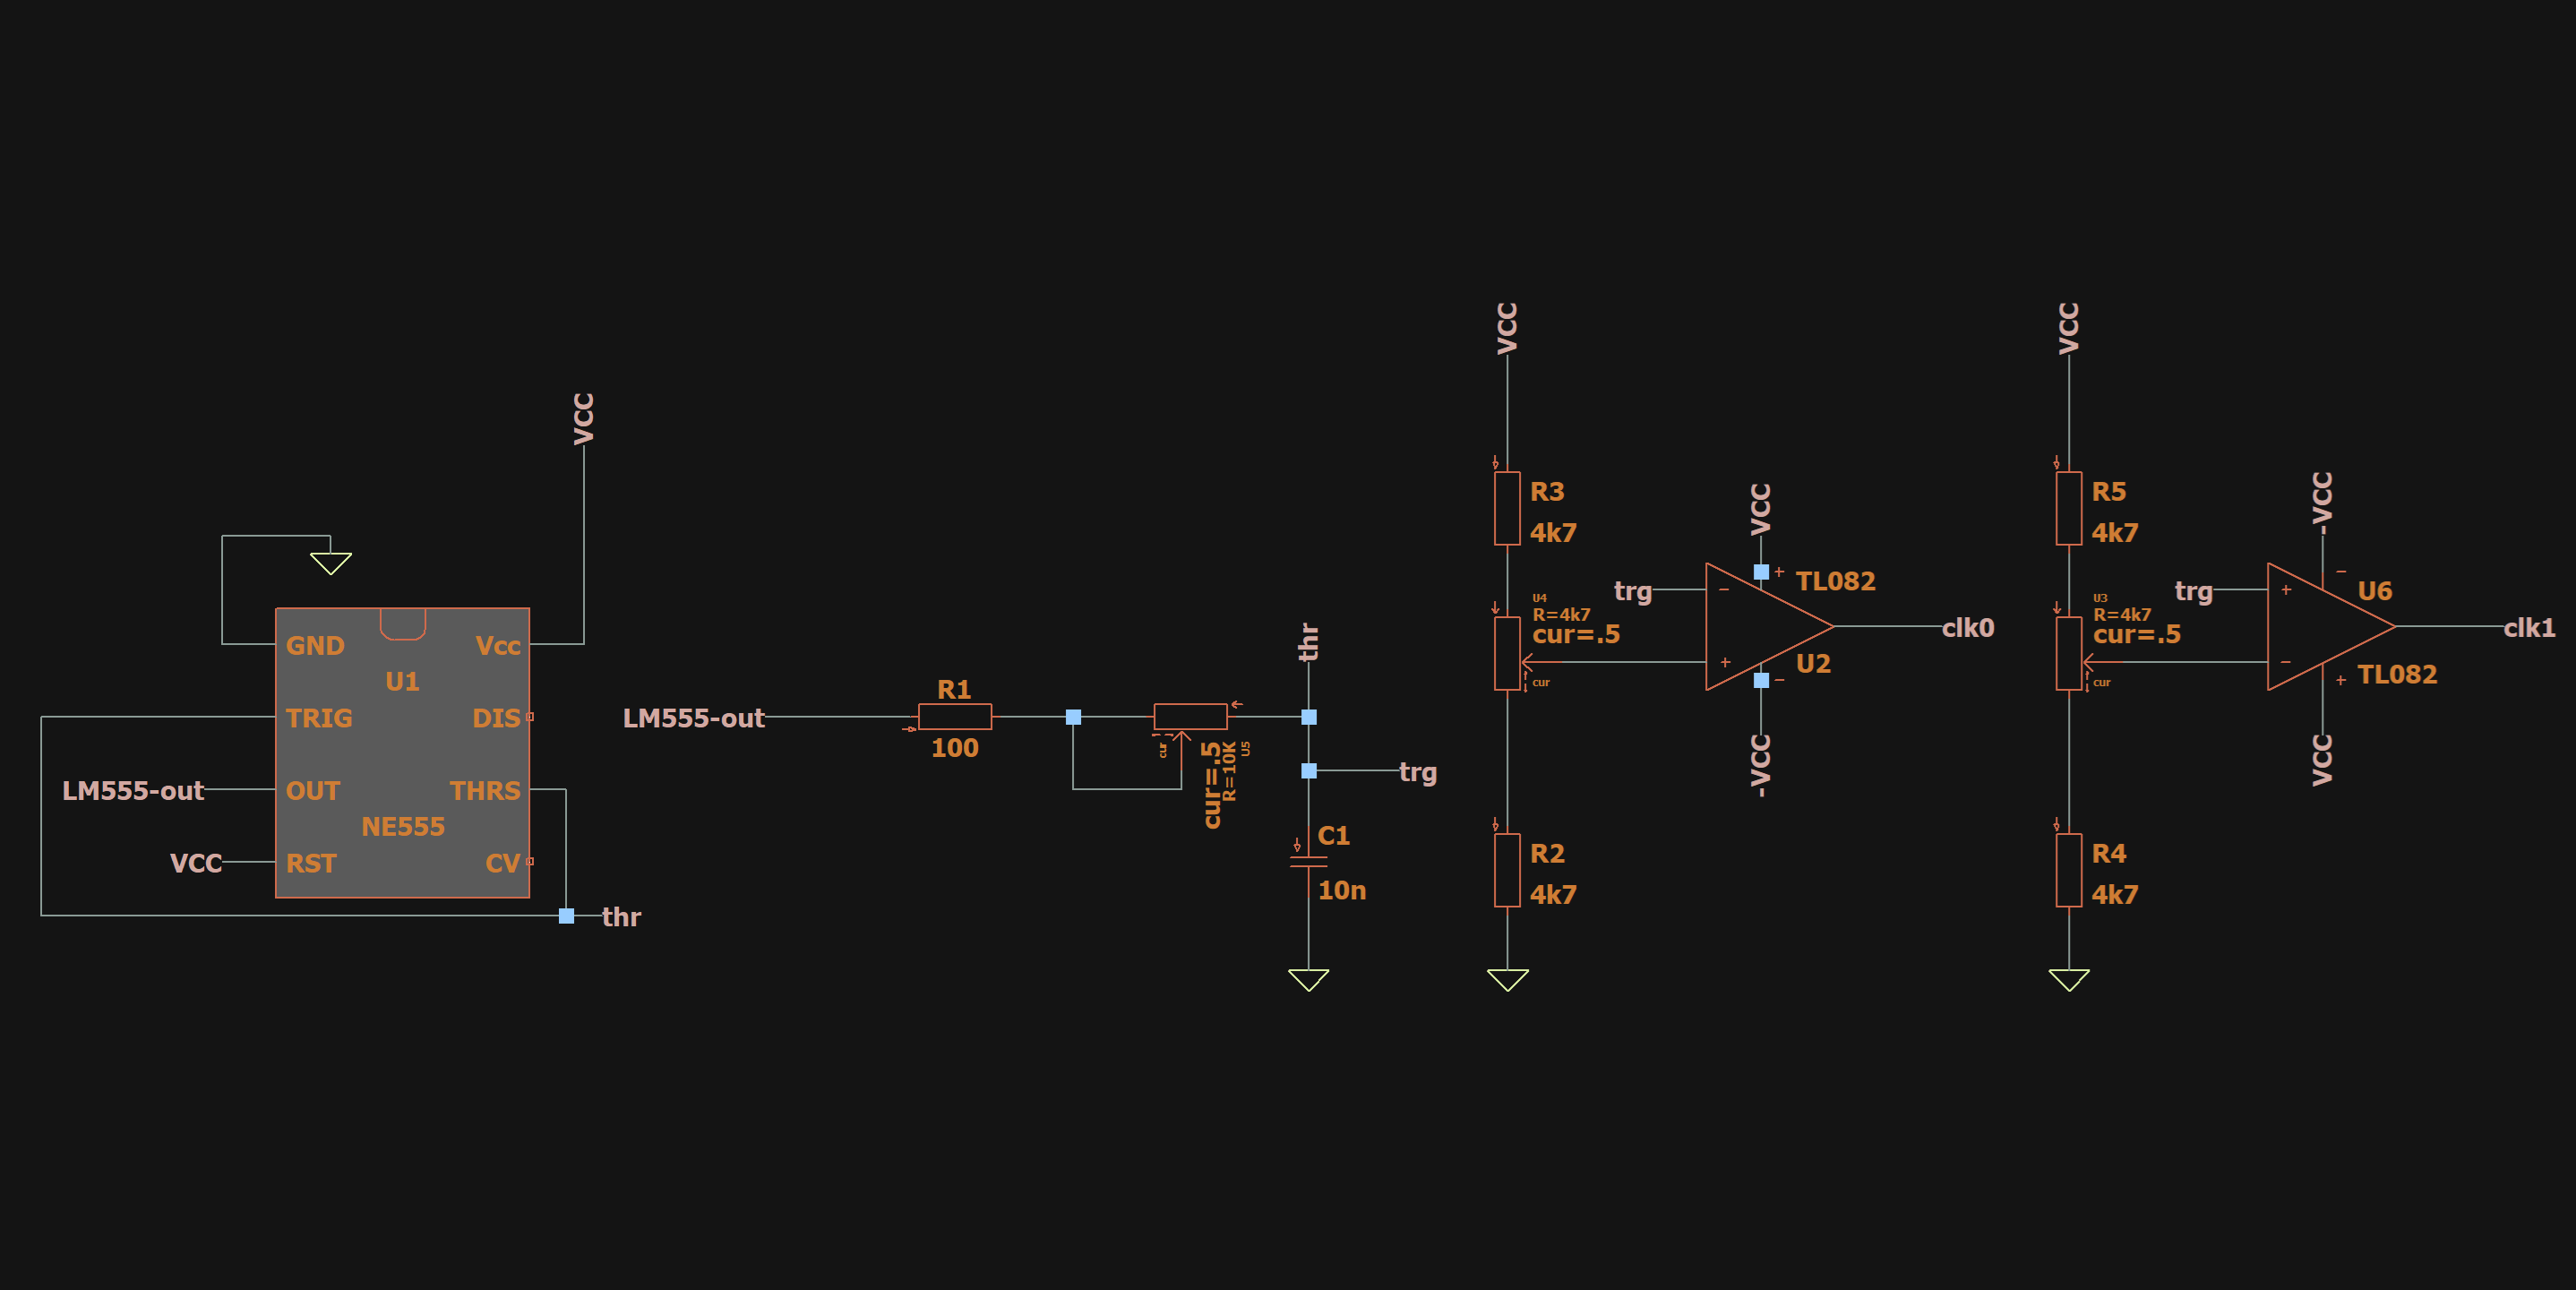
\includegraphics[width=0.8\linewidth]{Imagenes Nacho/OsciladorEsquema.png}
    \caption{Clocks del Sistema}
    \label{fig:OsciladorEsquema}
\end{figure}

\begin{figure}[H]
    \centering
    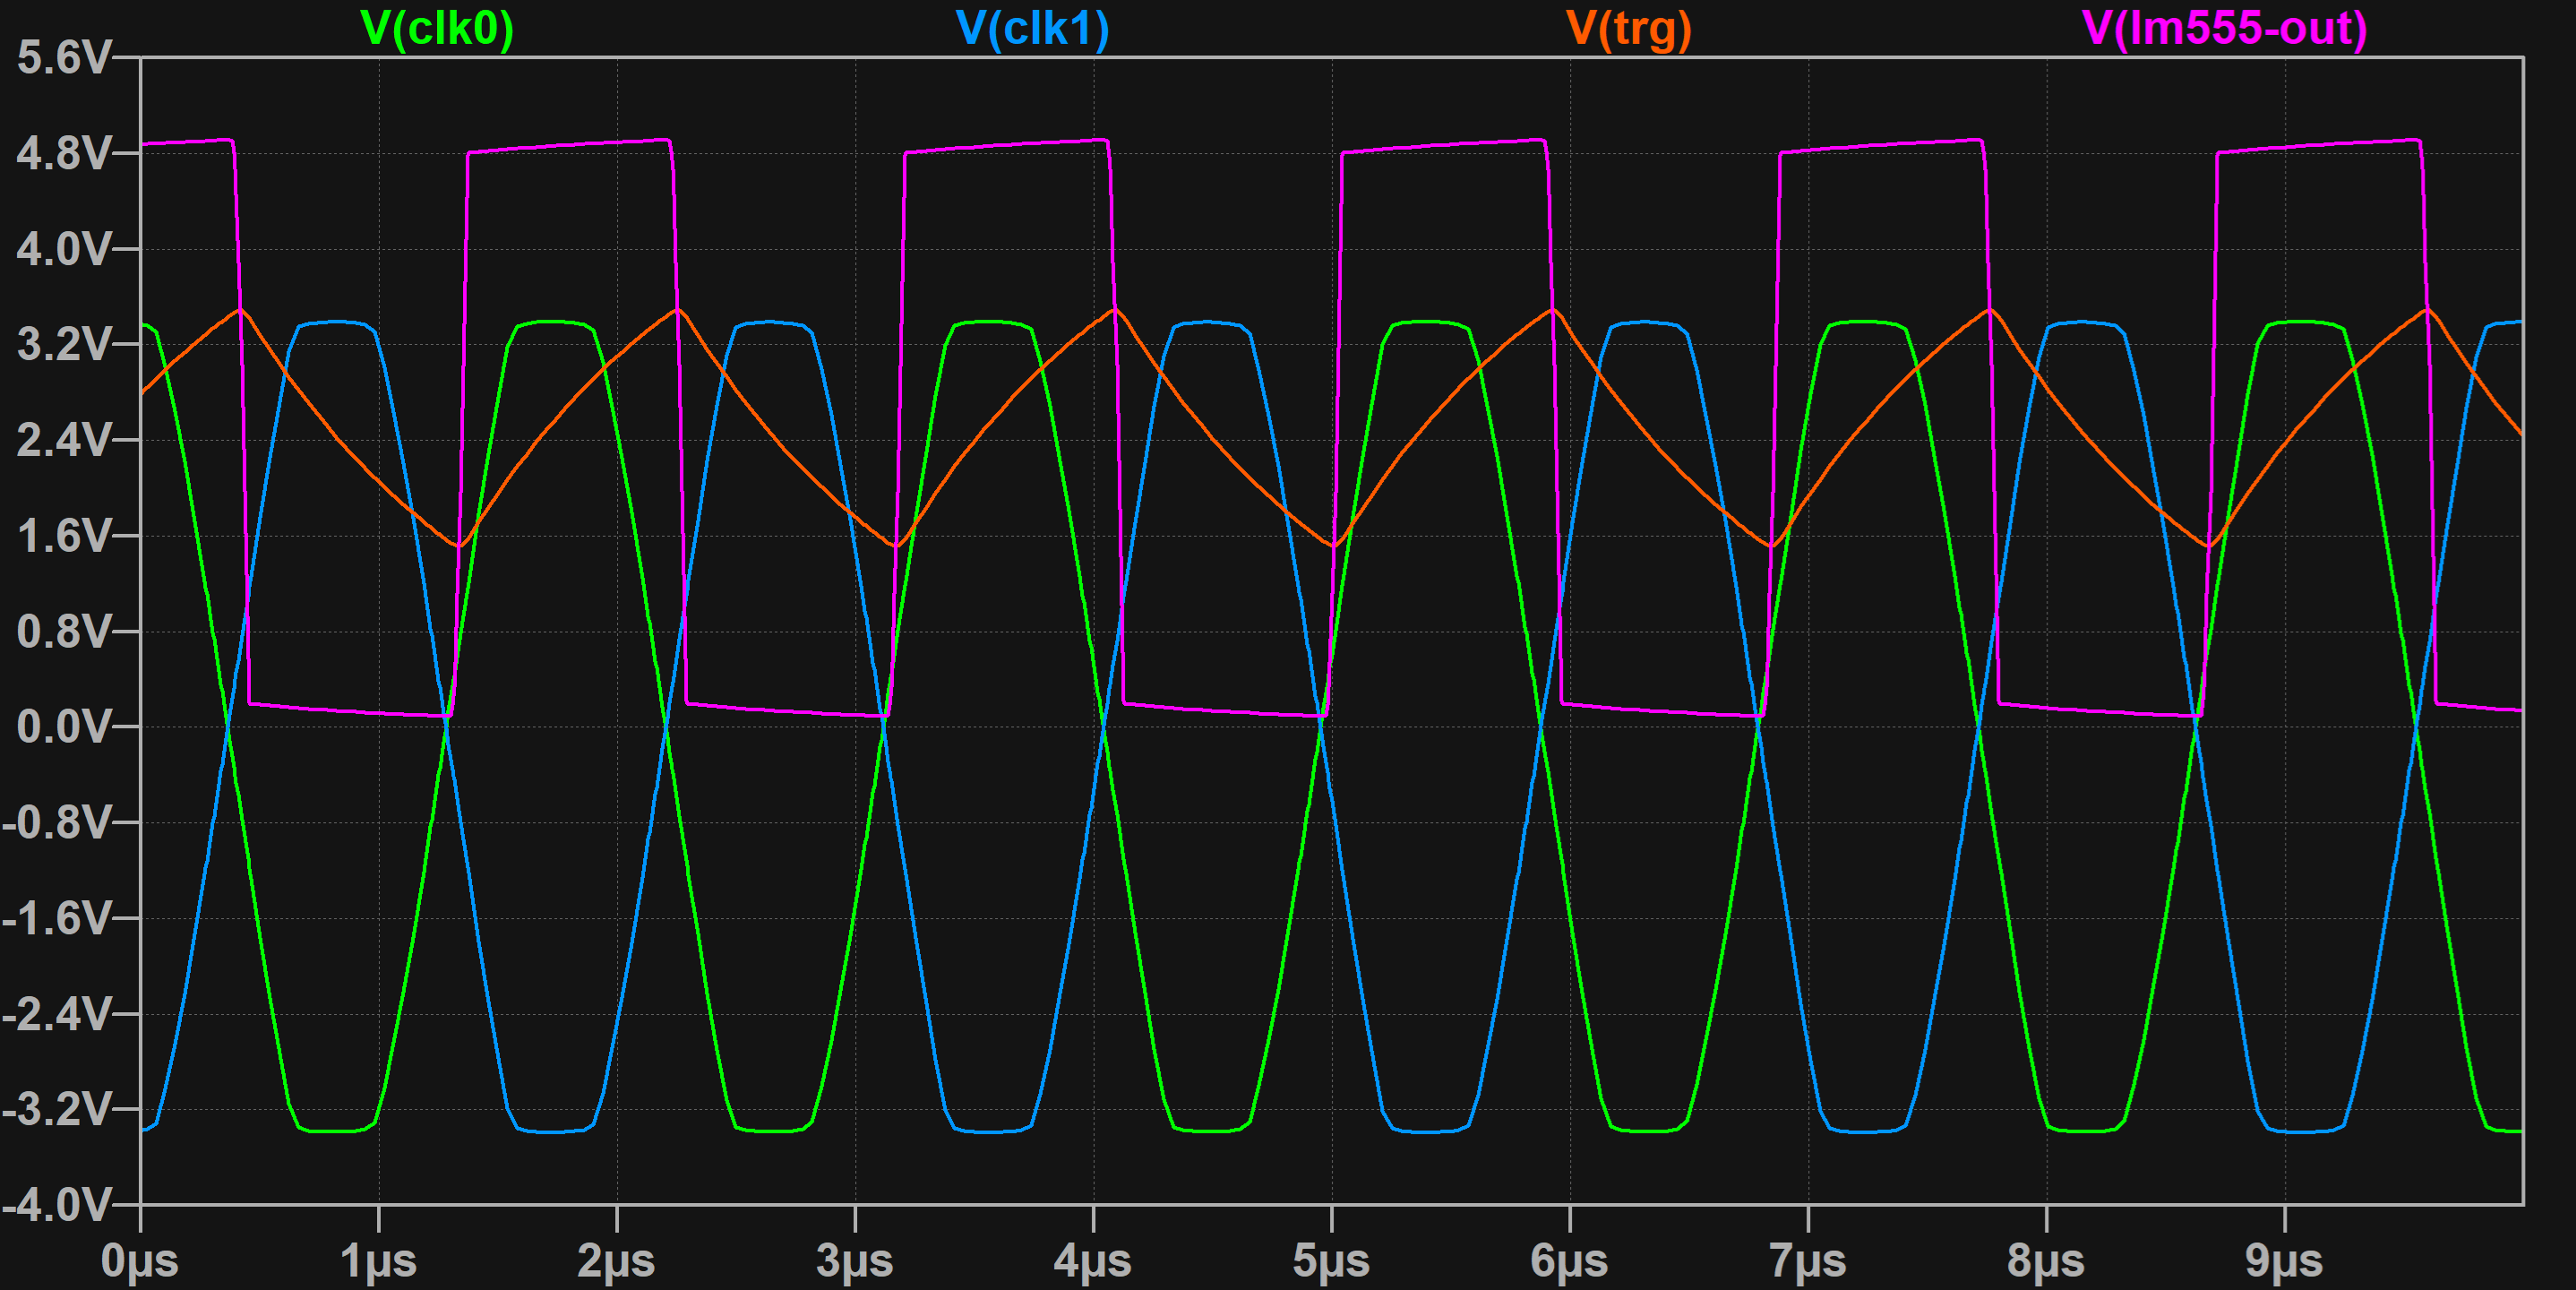
\includegraphics[width=0.8\linewidth]{Imagenes Nacho/Oscilador.png}
    \caption{Simulaci\'on de clock $250kHz$}
    \label{fig:Oscilador}
\end{figure}

\subsection{Simulaci\'on de Muestro Natural}
Muestreando una señal cuadrada de $f = 15kHz$ con $75\%$ de Duty Cycle a $f_s = 250kHz$ obtenemos los siguientes graficos:

\begin{figure}[H]
    \centering
    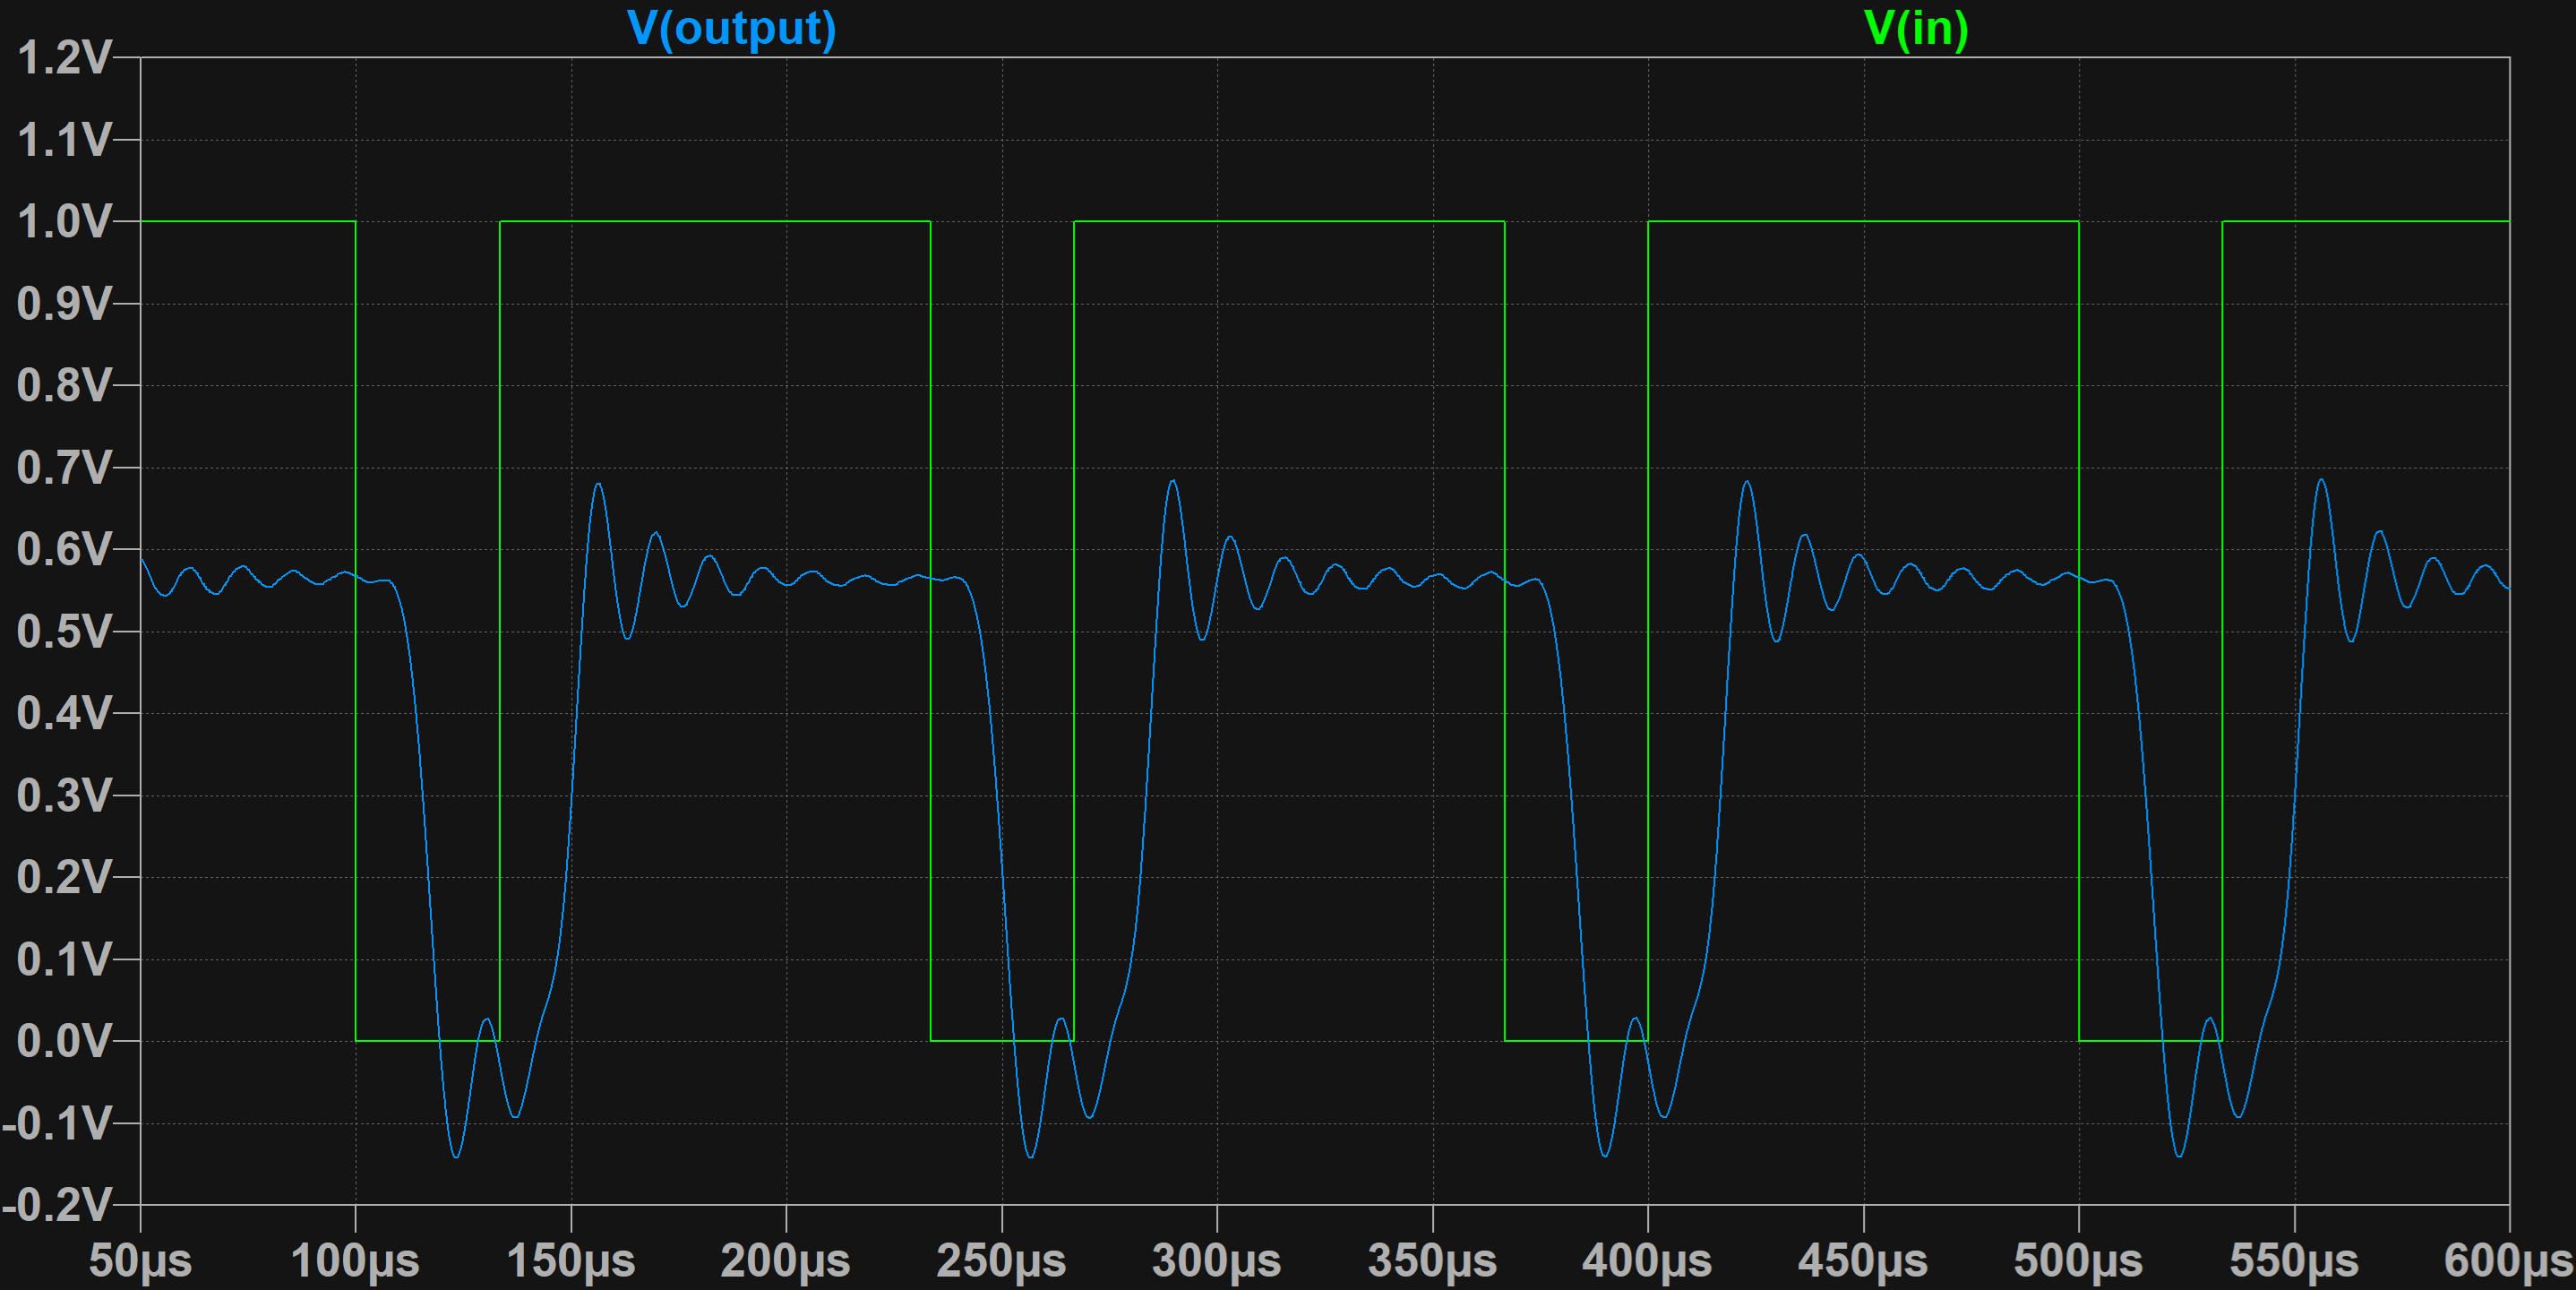
\includegraphics[width=0.8\linewidth]{Imagenes Nacho/Natural/Natural-Vi-Sqr15k.png}
    \caption{$V_o$ vs $V_i$}
    \label{fig:Natural-Vi-Sqr15k}
\end{figure}

\begin{figure}[H]
    \centering
    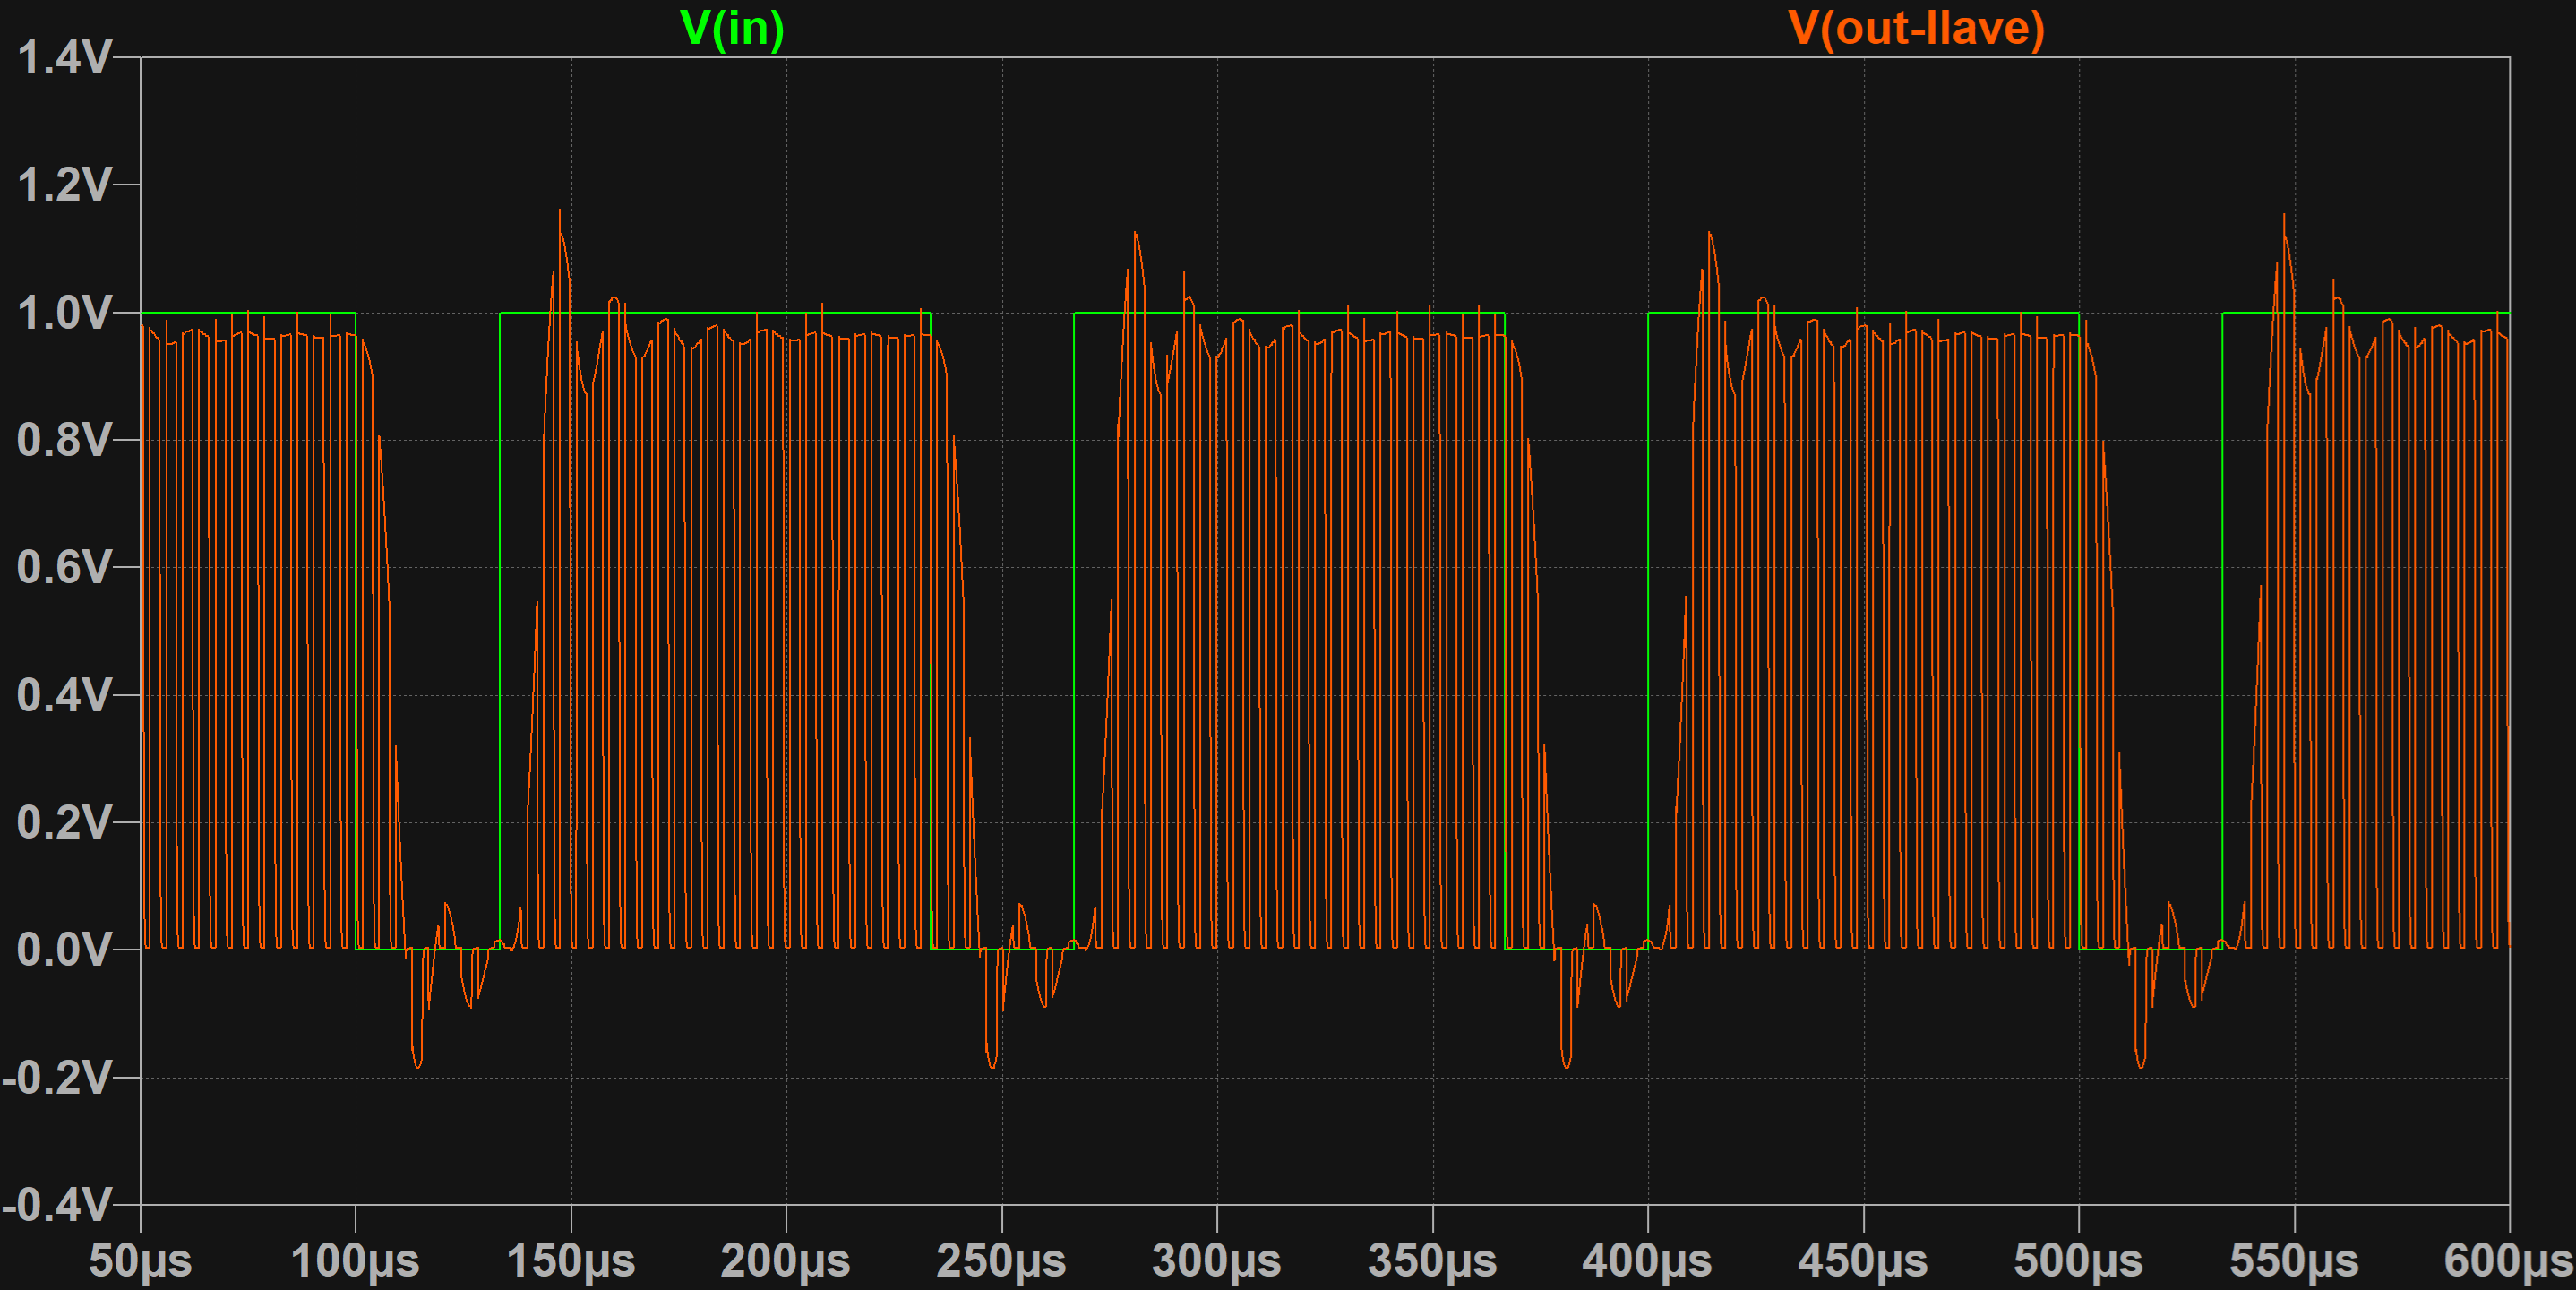
\includegraphics[width=0.8\linewidth]{Imagenes Nacho/Natural/Natural-Vi-Sqr15k-out-LLave.png}
    \caption{Salida de la llave vs $V_i$}
    \label{fig:out-LLave}
\end{figure}

\begin{figure}[H]
    \centering
    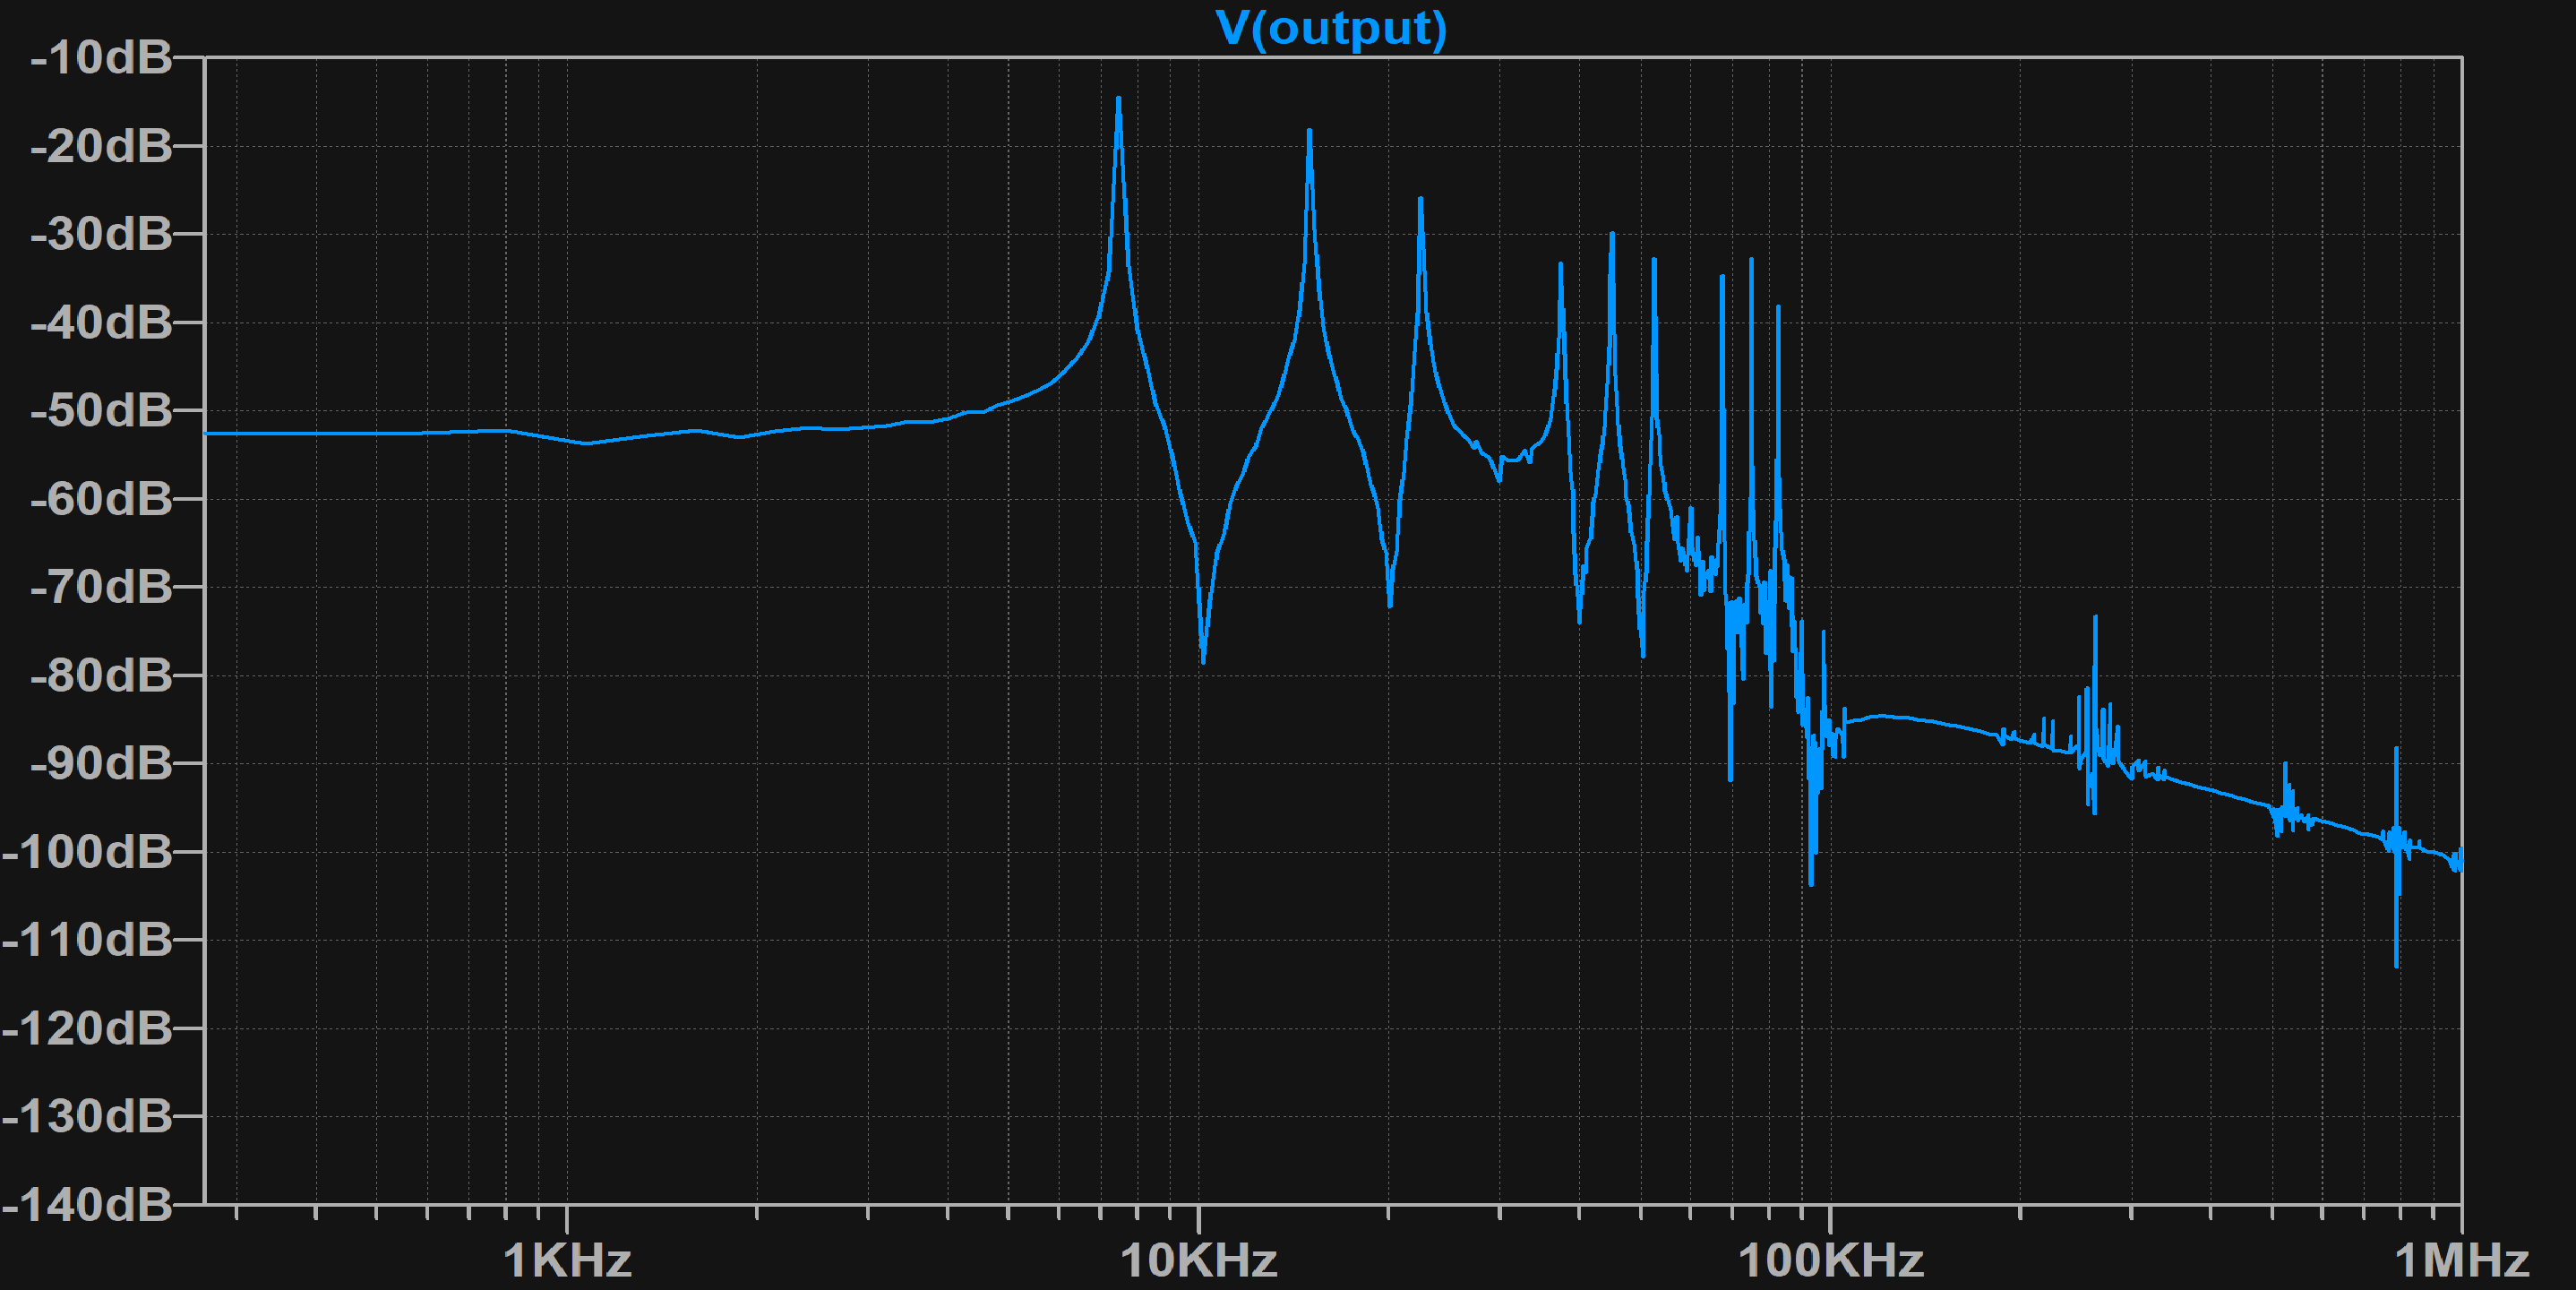
\includegraphics[width=0.8\linewidth]{Imagenes Nacho/Natural/Natural-Vi-Sqr15k-outFFT.png}
    \caption{FFT de la salida}
    \label{fig:FFT de la salida}
\end{figure}


\subsection{Simulaci\'on de Muestro Instantaneo}
Muestreando una señal cuadrada de $f = 15kHz$ con $75\%$ de Duty Cycle a $f_s = 250kHz$ obtenemos los siguientes graficos:

\begin{figure}[H]
    \centering
    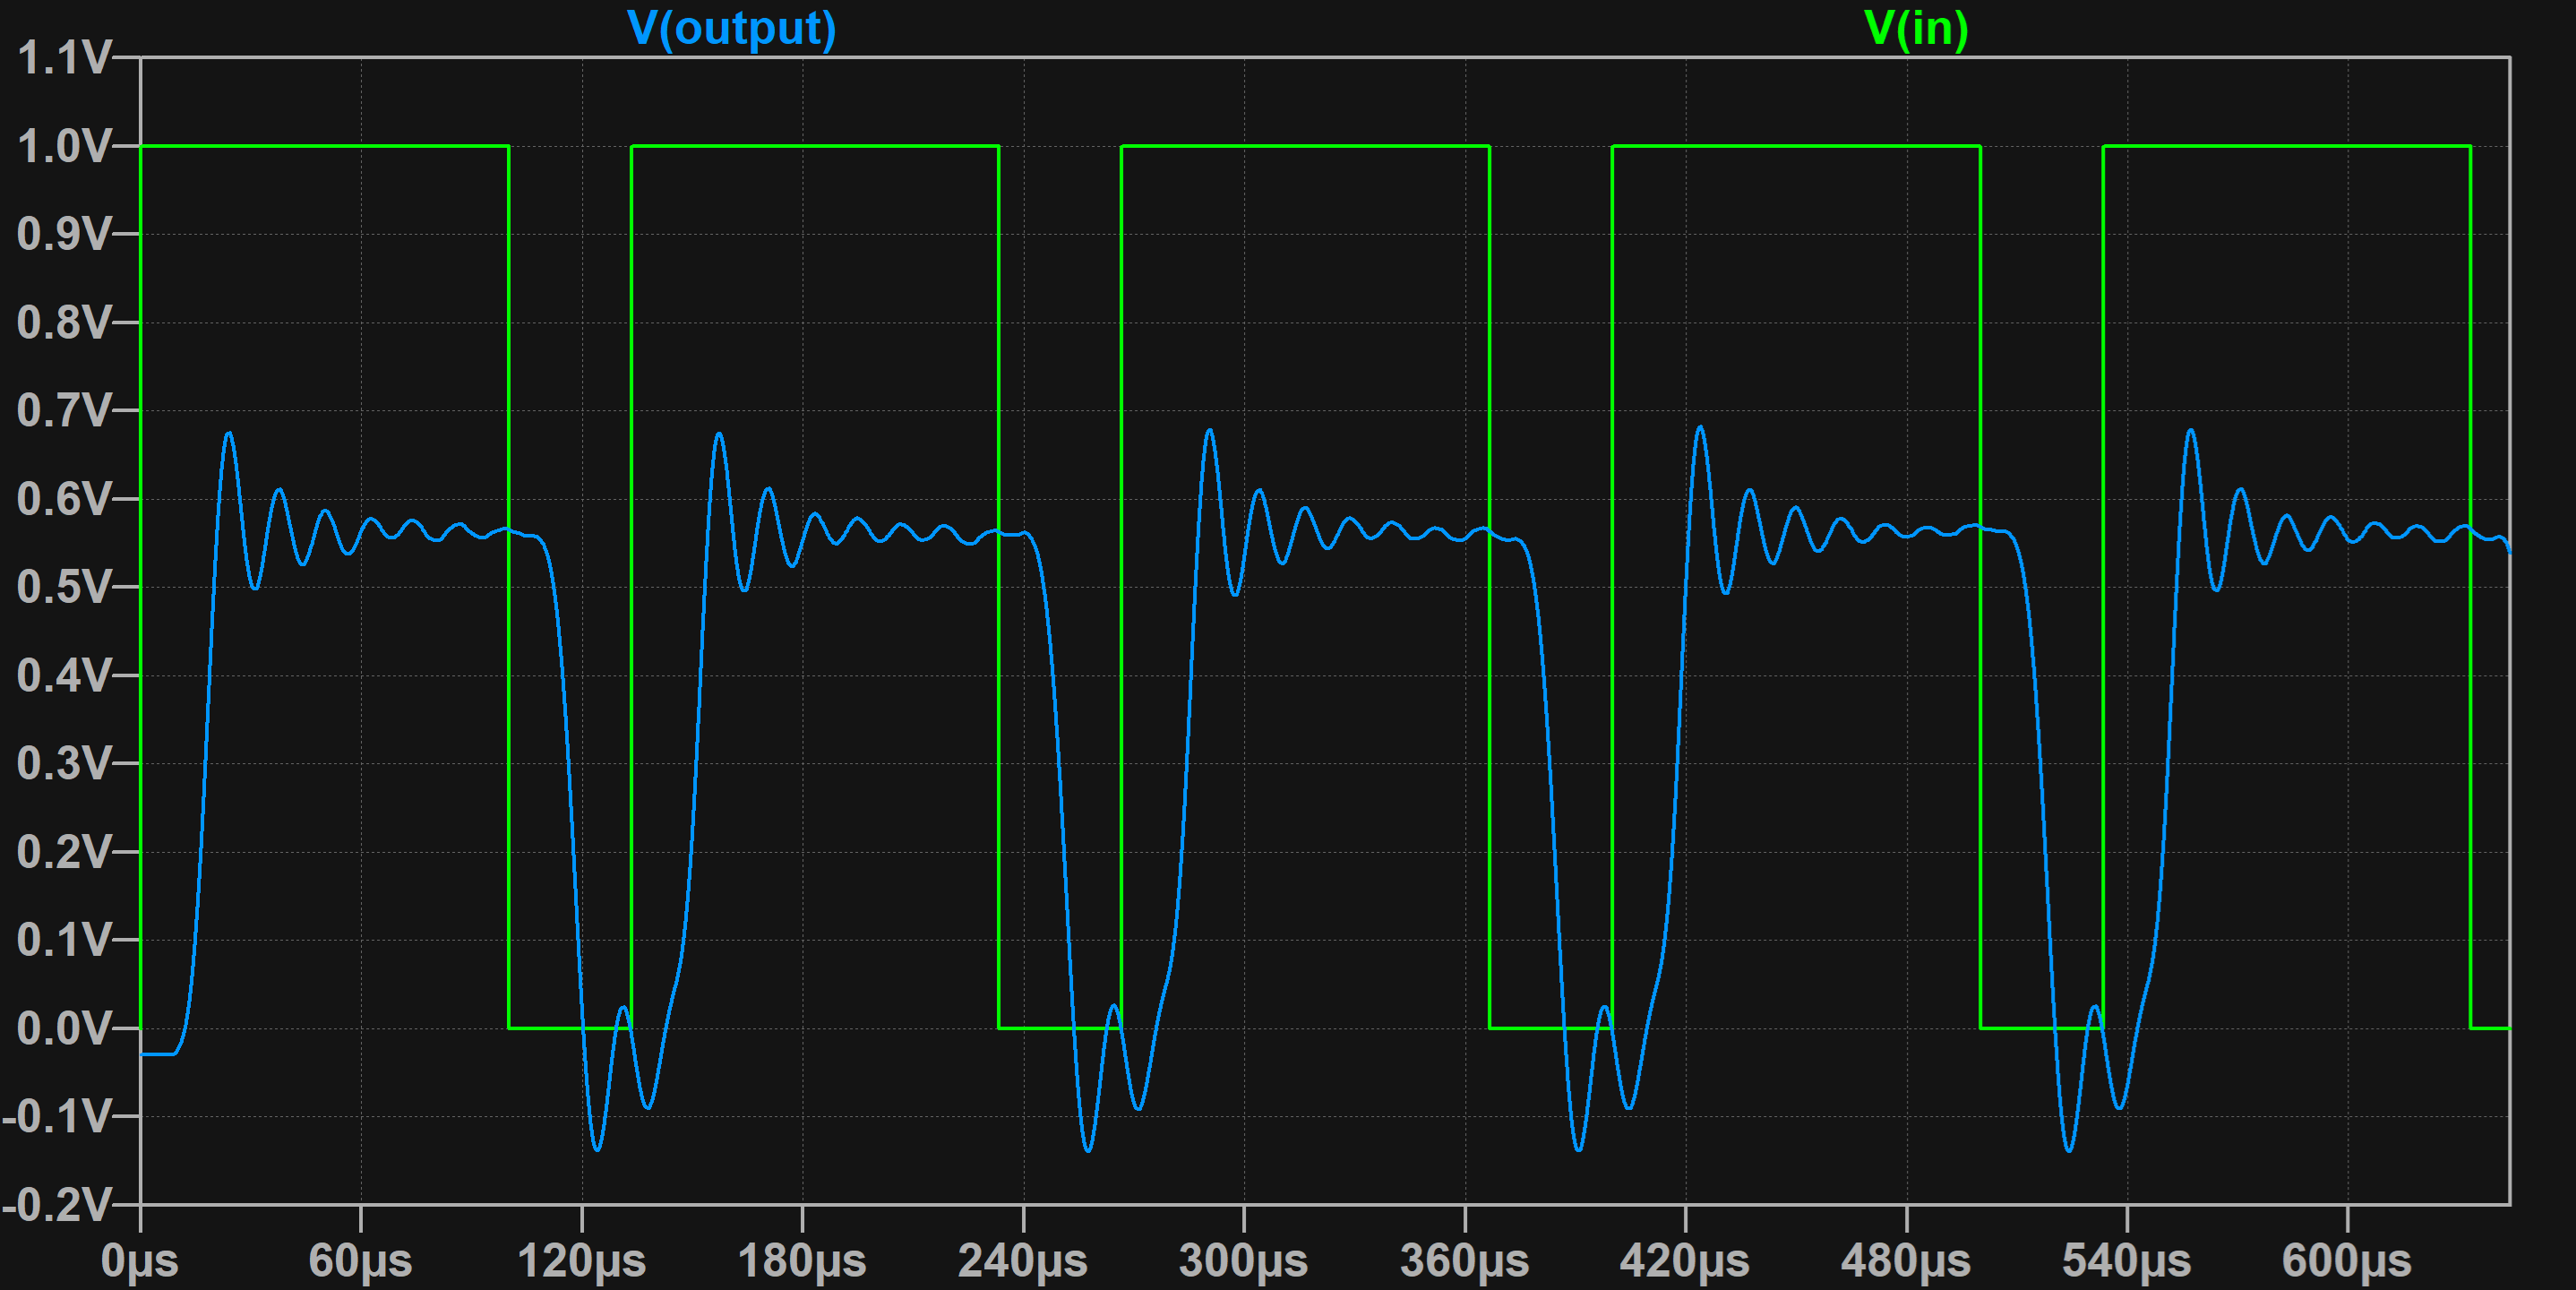
\includegraphics[width=0.8\linewidth]{Imagenes Nacho/Instantaneo/Vi-Vo.png}
    \caption{$V_o$ vs $V_i$}
    \label{fig:Vi-Vo}
\end{figure}

\begin{figure}[H]
    \centering
    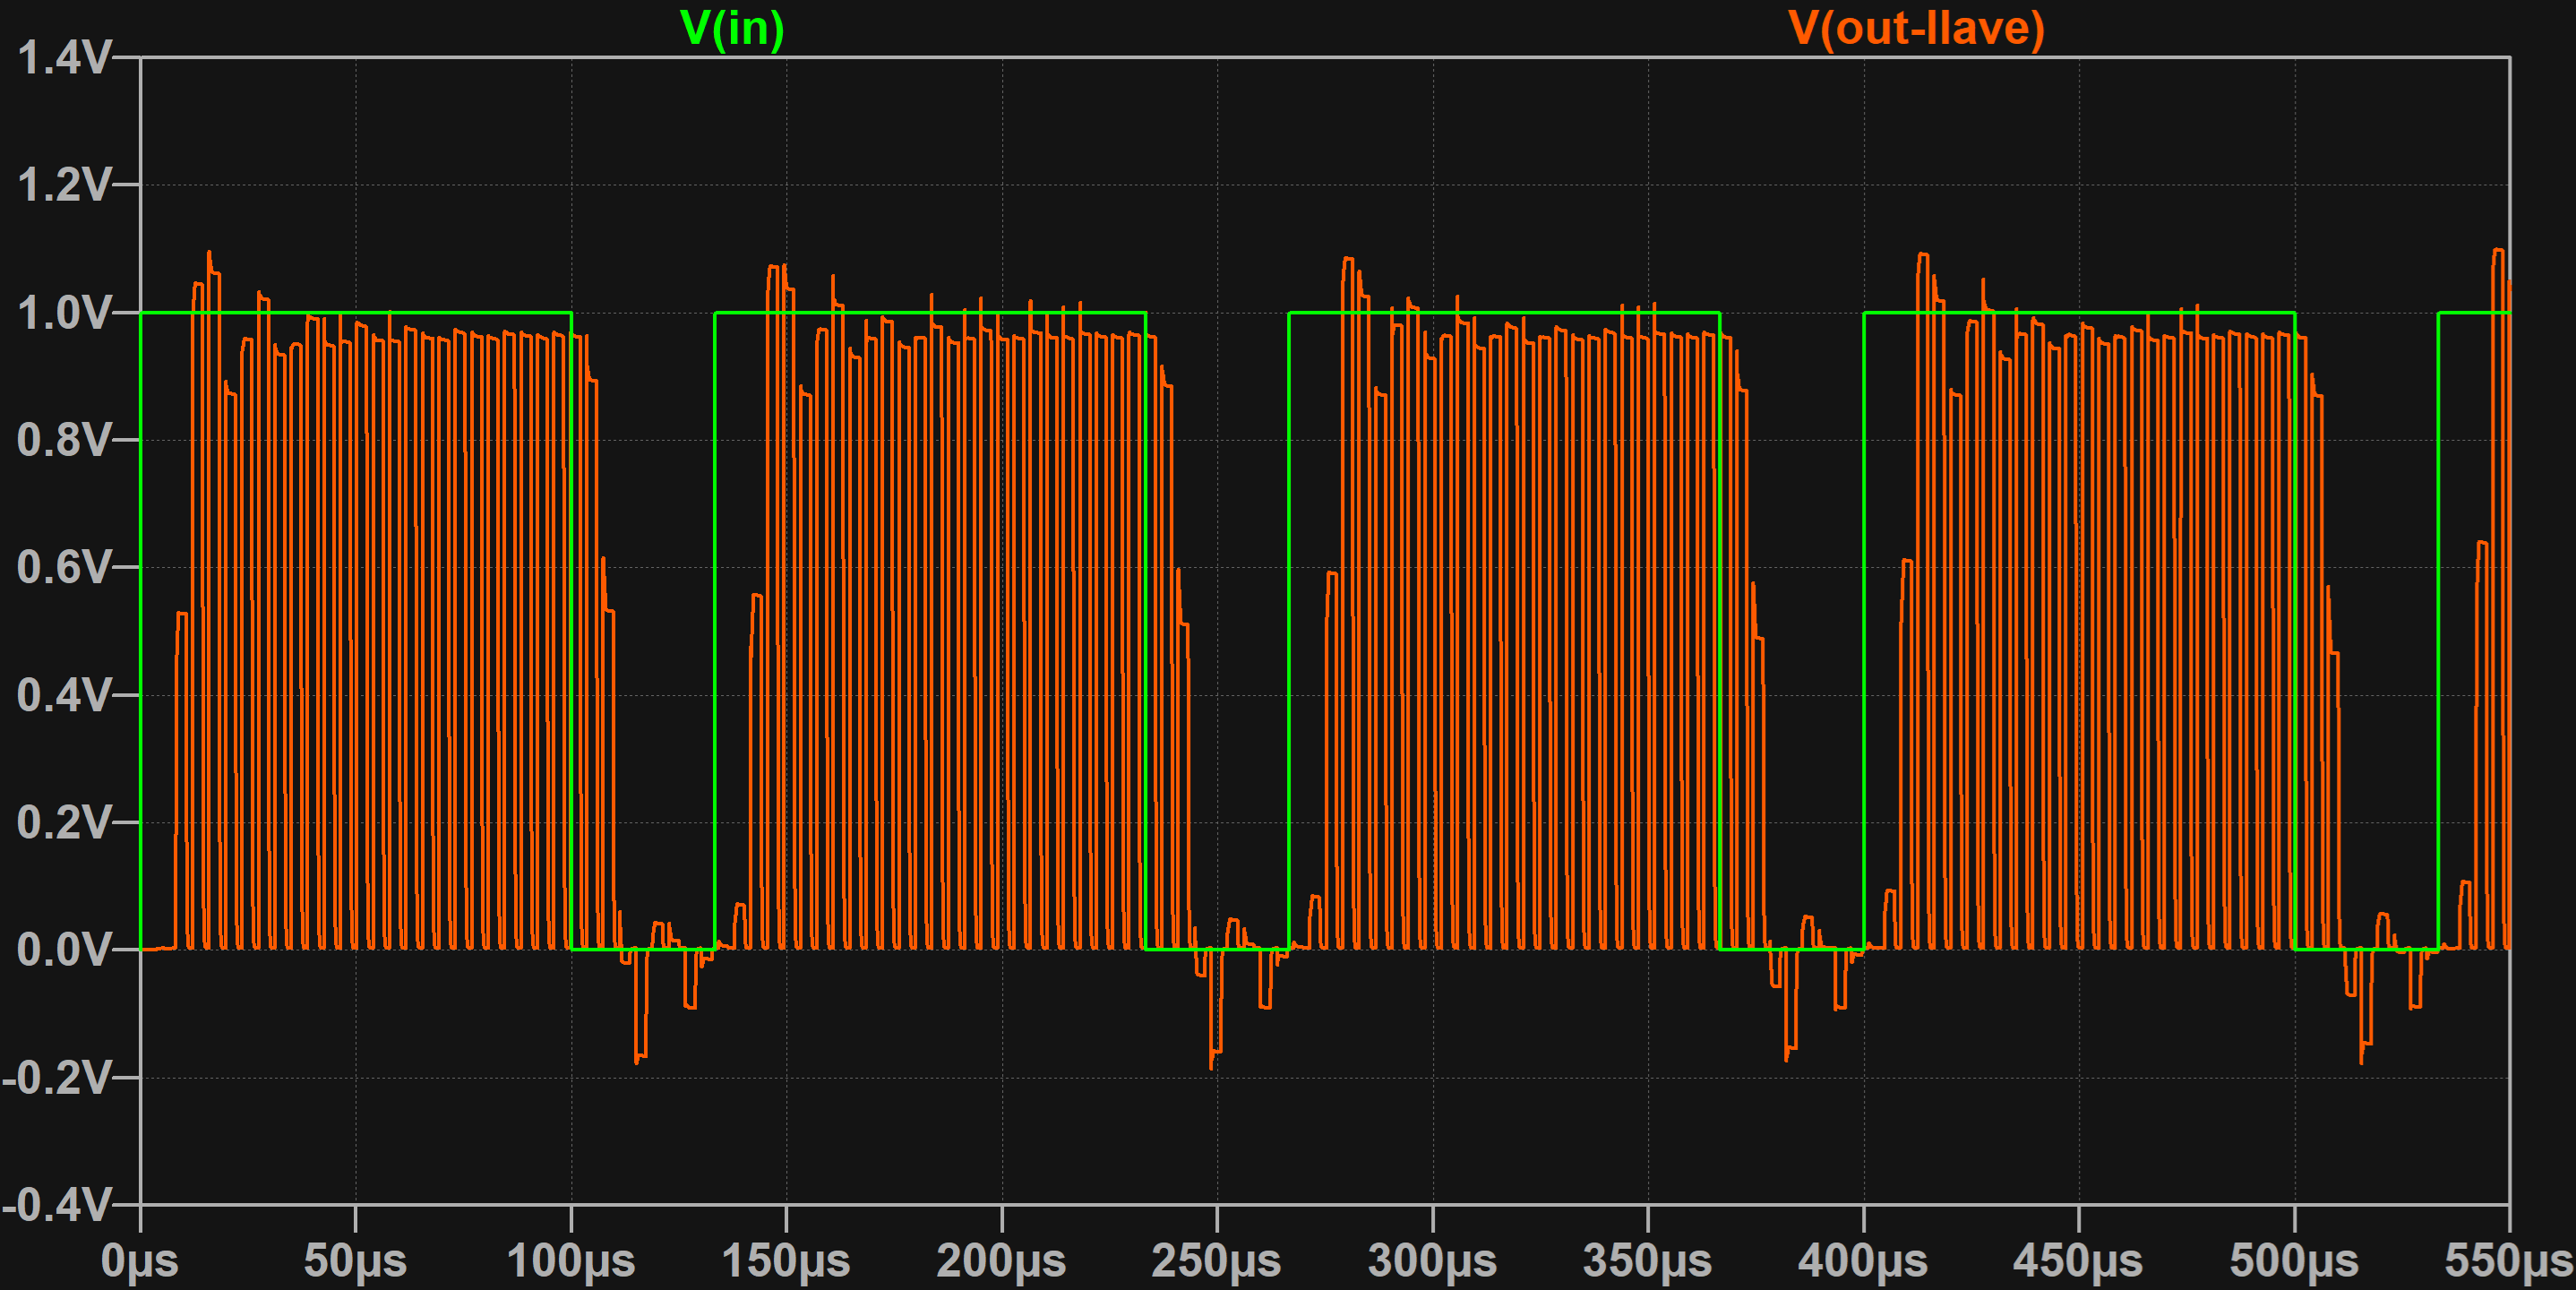
\includegraphics[width=0.8\linewidth]{Imagenes Nacho/Instantaneo/out-llave.png}
    \caption{Salida de la llave vs $V_i$}
    \label{fig:out-llave}
\end{figure}


\begin{figure}[H]
    \centering
    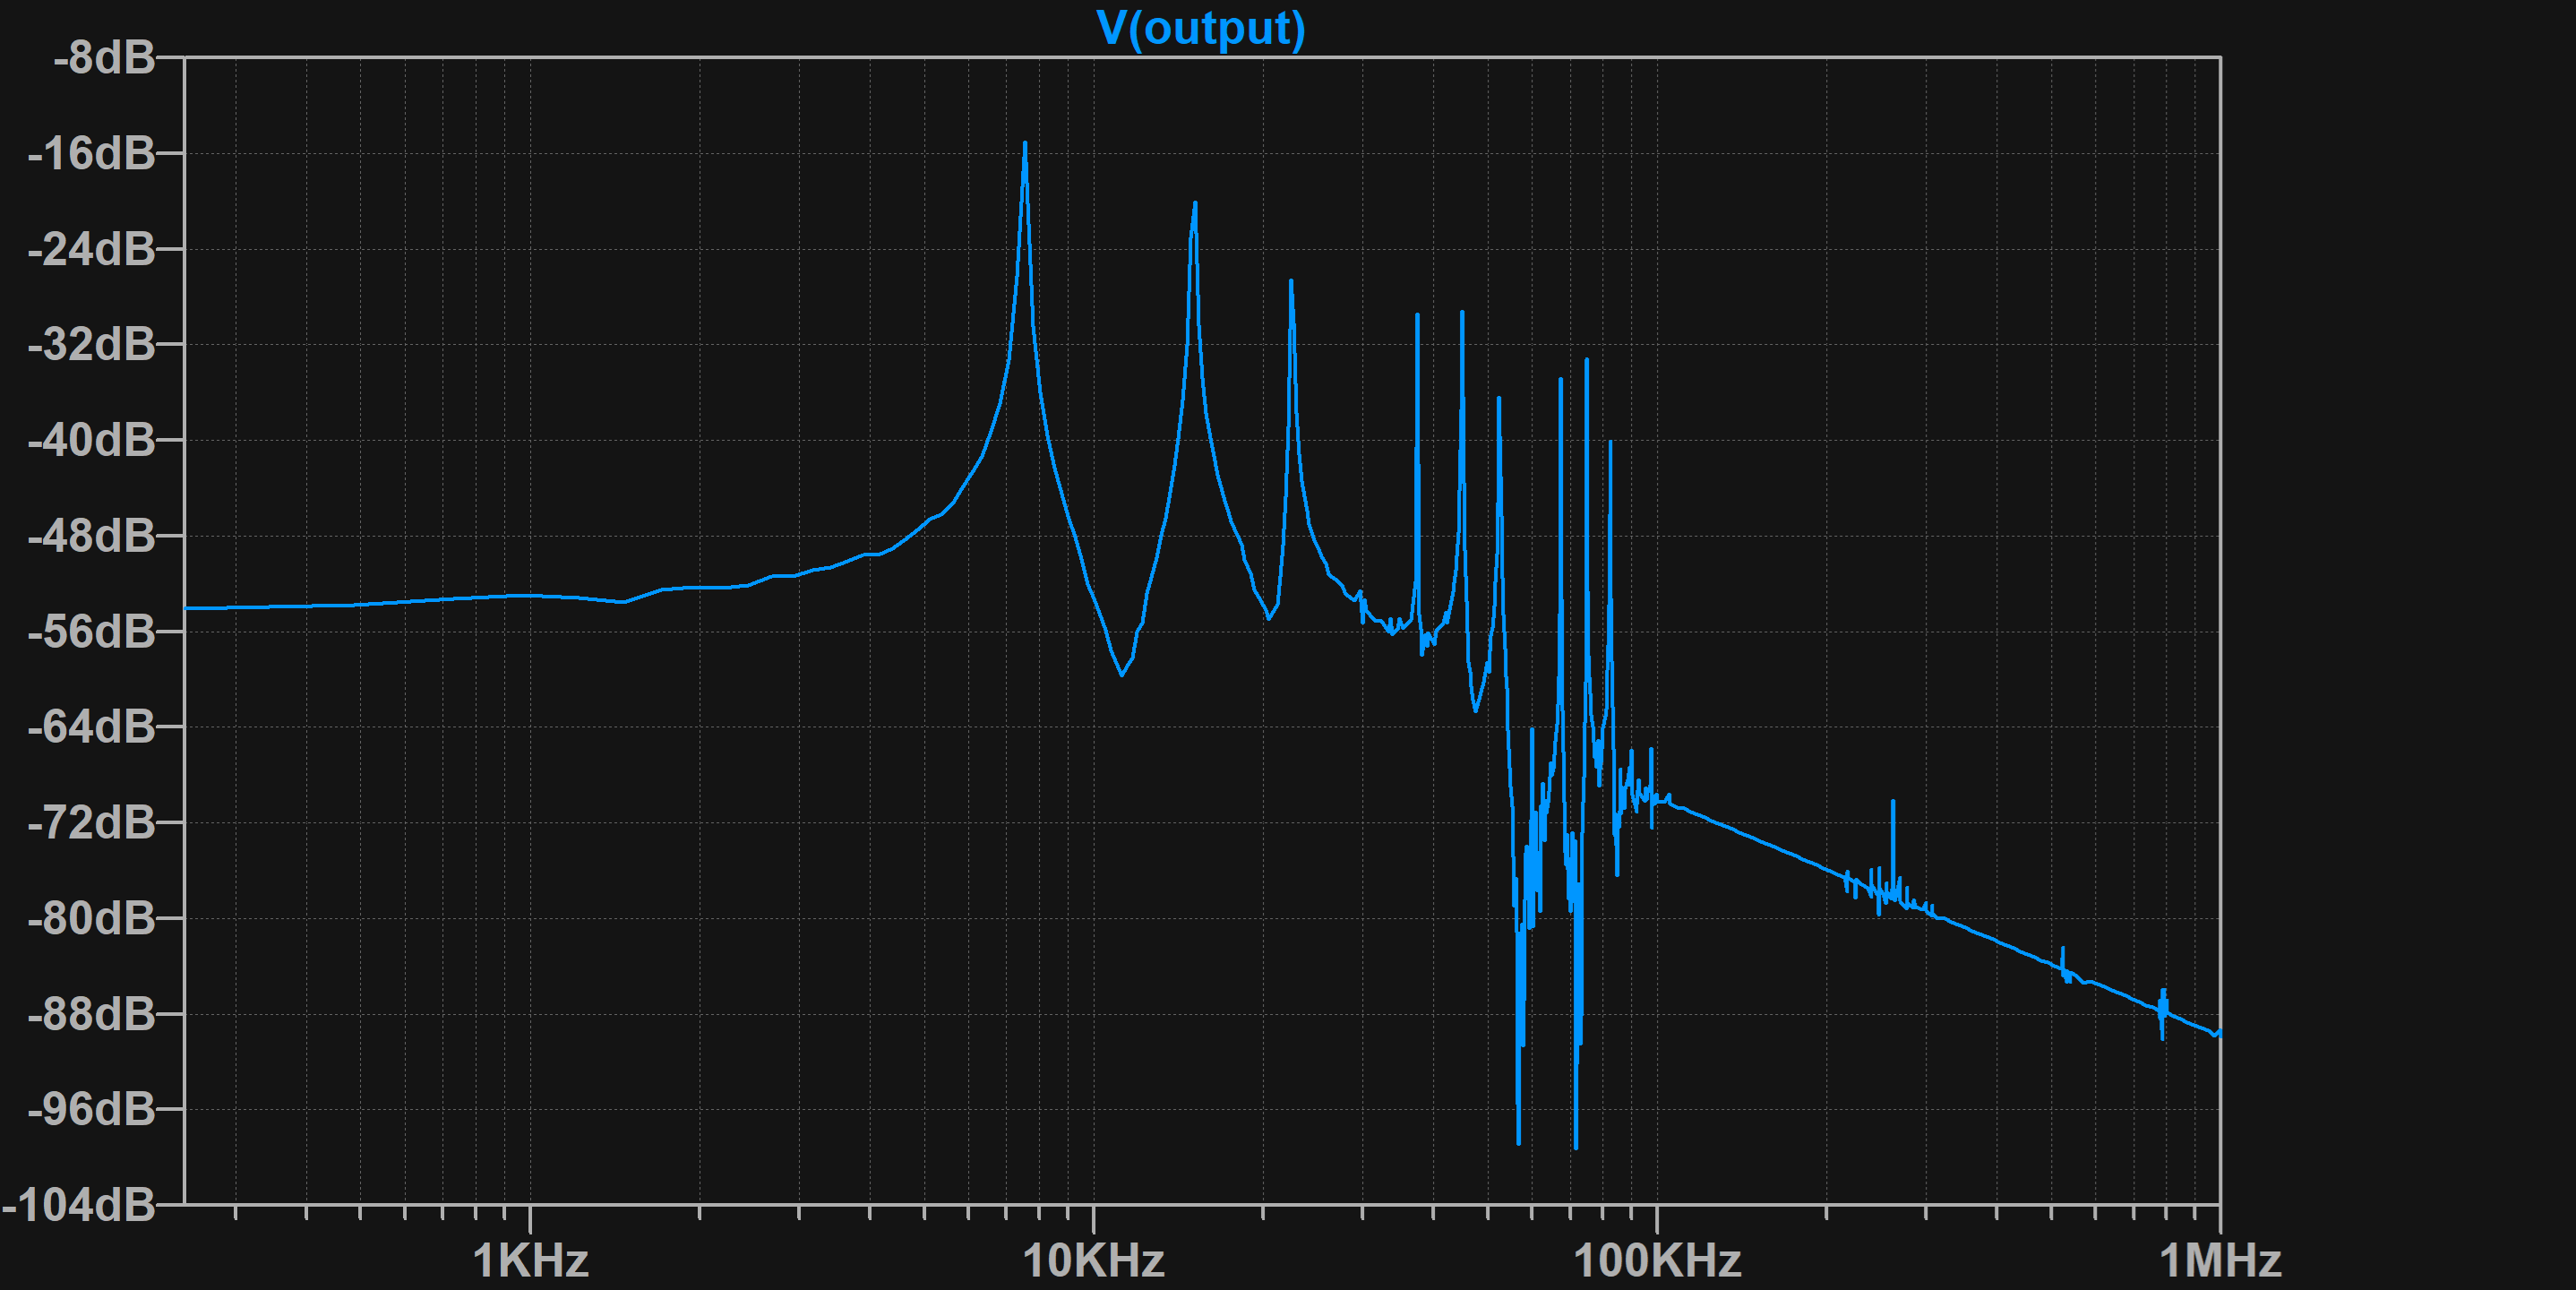
\includegraphics[width=0.8\linewidth]{Imagenes Nacho/Instantaneo/Vo-FFT.png}
    \caption{FFT de $V_o$}
    \label{fig:FFT}
\end{figure}

